%%%%%%%%%%%%%%%%%%%%%%%%%%%%%%%%%%%%%%%%%%%%%%%%%%%%%%%%%%%%
% preferences
%%%%%%%%%%%%%%%%%%%%%%%%%%%%%%%%%%%%%%%%%%%%%%%%%%%%%%%%%%%%
\documentclass[a4j,10pt,uplatex]{jsbook}	% class の指定
%%%%%%%%%%%%%%%%%%%%%%%%%%%%%%%%%%%%%%%%%%%%%%%%%%%%%%%%%%%%%
% package setting
%%%%%%%%%%%%%%%%%%%%%%%%%%%%%%%%%%%%%%%%%%%%%%%%%%%%%%%%%%%%
\usepackage[dvipdfmx, colorlinks=false, bookmarks=true, bookmarksnumbered=false, pdfborder={0 0 0}, bookmarkstype=toc]{hyperref}
\usepackage{pxjahyper}				% 上と合わせて栞とリンクの設定
\usepackage{amsmath, amssymb}		% アメリカ数学会(AMS)開発の数式記号
\usepackage[dvipdfmx]{graphicx}		% 画像の読み込み
\usepackage{float}					% H で画像を指定の位置に配置
\usepackage{multicol}				% 表のセルの横方向の結合
\usepackage{multirow}				% 表のセルの縦方向の結合
\usepackage{url}					% URL の記載  \url{...}
\usepackage{comment}				% コメントアウトの範囲指定  \begin{comment} ~ \end{comment}


%%%%%%%%%%%%%%%%%%%%%%%%%%%%%%%%%%%%%%%%%%%%%%%%%%%%%%%%%%%%
% command setting
%%%%%%%%%%%%%%%%%%%%%%%%%%%%%%%%%%%%%%%%%%%%%%%%%%%%%%%%%%%%
\newcommand{\Fe}{$\rm ^{55}Fe$}
\newcommand{\Co}{$\rm ^{57}Co$}
\newcommand{\Cd}{$\rm ^{109}Cd$}
\newcommand{\Am}{$\rm ^{241}Am$}					% 森研のパッケージ・コマンドのテンプレートの読み込み
%%%%%%%%%%%%%%%%%%%%%%%%%%%%%%%%%%%%%%%%%%%%%%%%%%%%%%%%%%%%
% package setting
%%%%%%%%%%%%%%%%%%%%%%%%%%%%%%%%%%%%%%%%%%%%%%%%%%%%%%%%%%%%
\usepackage[dvipdfmx, colorlinks=false, bookmarks=true, bookmarksnumbered=false, pdfborder={0 0 0}, bookmarkstype=toc]{hyperref}
\usepackage{pxjahyper}				% 上と合わせて栞とリンクの設定
\usepackage{amsmath, amssymb}		% アメリカ数学会(AMS)開発の数式記号
\usepackage[dvipdfmx]{graphicx}		% 画像の読み込み
\usepackage{float}					% H で画像を指定の位置に配置
\usepackage{multicol}				% 表のセルの横方向の結合
\usepackage{multirow}				% 表のセルの縦方向の結合
\usepackage{url}					% URL の記載  \url{...}
\usepackage{comment}				% コメントアウトの範囲指定  \begin{comment} ~ \end{comment}


%%%%%%%%%%%%%%%%%%%%%%%%%%%%%%%%%%%%%%%%%%%%%%%%%%%%%%%%%%%%
% command setting
%%%%%%%%%%%%%%%%%%%%%%%%%%%%%%%%%%%%%%%%%%%%%%%%%%%%%%%%%%%%
\newcommand{\Fe}{$\rm ^{55}Fe$}
\newcommand{\Co}{$\rm ^{57}Co$}
\newcommand{\Cd}{$\rm ^{109}Cd$}
\newcommand{\Am}{$\rm ^{241}Am$}

\oddsidemargin -7.4mm						% 奇数ページの左の余白
\evensidemargin -7.4mm						% 偶数ページの左の余白
\textwidth 174mm							% 1 行の幅
\topmargin 0mm 								% 上の余白
\headheight 0pt								% ヘッダの縦幅
\headsep 25pt								% ページ数と本文の間
\textheight 246mm							% 本文の縦幅
\parindent 1pt								% 改段落時の字下げ幅
\columnsep 0mm								% 段組み間の幅
\baselineskip 14pt plus 1pt minus 1pt		% 行間の設定


%%%%%%%%%%%%%%%%%%%%%%%%%%%%%%%%%%%%%%%%%%%%%%%%%%%%%%%%%%%%
% Cover Page
%%%%%%%%%%%%%%%%%%%%%%%%%%%%%%%%%%%%%%%%%%%%%%%%%%%%%%%%%%%%
\begin{document}

\title{
令和6年度 卒業論文\\
\vspace{4ex}
\huge \mbox{X線分光撮像衛星 XRISM に搭載した} \mbox{軟X線撮像検出器 SXI による}\mbox{太陽フレアの地球大気反射X線の観測}}


\author{
宮崎大学 工学部 工学科 応用物理工学プログラム\\
%宮崎大学 工学研究科 工学専攻 エネルギー系コース\\
\\
\Large{倉嶋 順}\\
}

\date{\today}
\maketitle


%%%%%%%%%%%%%%%%%%%%%%%%%%%%%%%%%%%%%%%%%%%%%%%%%%%%%%%%%%%%
% Abstract
%%%%%%%%%%%%%%%%%%%%%%%%%%%%%%%%%%%%%%%%%%%%%%%%%%%%%%%%%%%%
\section*{Abstract}

本研究では、X線分光撮像衛星 XRISM に搭載した 軟X線撮像検出器 SXI を用いて、\mbox{2023年10月19日}から\mbox{2024年12月31日}の期間における、太陽フレアの地球大気反射X線 の観測を行った。太陽活動の極大期により、\mbox{2024年}に大規模な太陽フレアが頻繁に発生し、XRISM /SXI でも多数のフレアを観測した。観測したフレアから、フレアピーク付近を観測した9つのフレアを解析に使用した。まず、9つのフレアを足し合わせた積分スペクトルを作成した。フレアの積分スペクトルから、Si, S, Ar, Ca, Ti, Cr, Fe, Ni の輝線を検出した。Katsuda et al. 2020\cite{Katsuda}と比較して、新たに Ti, Cr, Ni の輝線が得られた。次に、フレアクラス別に Si, S, Ar, Ca, Fe の絶対元素組成比の測定を行った。測定の結果、すべてのフレアで、Katsuda et al. 2020\cite{Katsuda}と同様に、活動的な恒星コロナに見られる i-FIP 効果に類似する絶対元素組成比パターンが得られた。また、本研究で新たに、Fe の絶対元素組成比の測定を行った結果、ほぼ全てのフレアにおける絶対元素組成比が 0.76-1.37 であった。これは、FIP の近い Si の絶対元素組成比と同様の結果であり、恒星コロナの FIP 効果と i-FIP 効果を説明する  Laming model (Laming et al, 2021\cite{Laming_2021})と整合している。最後に、フレアピーク付近における絶対元素組成比の時間変動を検証した。Si , S, Ca の絶対元素組成比は、フレアの立ち上がりから、フレアピークにかけて増大し、フレアピーク以降は減少している傾向が見られた。特に Ca はフレアピーク付近で顕著に変動することが明らかとなった。


%%%%%%%%%%%%%%%%%%%%%%%%%%%%%%%%%%%%%%%%%%%%%%%%%%%%%%%%%%%%
% List of Contents, Figures and Tables
%%%%%%%%%%%%%%%%%%%%%%%%%%%%%%%%%%%%%%%%%%%%%%%%%%%%%%%%%%%%
%\dominitoc
%\dominilof
%\dominilot
\setcounter{tocdepth}{3}
\tableofcontents
%\listoffigures
%\listoftables
\clearpage


%%%%%%%%%%%%%%%%%%%%%%%%%%%%%%%%%%%%%%%%%%%%%%%%%%%%%%%%%%%%
% Main Text
%%%%%%%%%%%%%%%%%%%%%%%%%%%%%%%%%%%%%%%%%%%%%%%%%%%%%%%%%%%%
\chapter{Introduction}

\section{研究背景}



20世紀後半、太陽大気コロナの極端紫外線およびX線分光観測、さらには太陽光エネルギー粒子や太陽風の直接観測により、太陽コロナの元素組成比が下層の光球と異なることが明らかになった。この違いは、元素の第一イオン化ポテンシャル(First Ionization Potential, FIP)に依存することによって説明されている(e.g.,Meyer 1985\cite{Meyer};Schmelz et al.2012\cite{Schmelz};Reames 2018\cite{Reames})。コロナでは、FIPが低い元素($\gtrsim10$)は、光球の元素組成比と比較して2倍から4倍に増加している(e.g.,Feldman 1992\cite{Feldman}; Dennis et al. 2015\cite{Dennis})。これは広く``FIP効果''として知られているが、そのメカニズムは、太陽物理学におけるコロナ加熱問題と並ぶ、長年の未解決問題の一つである。
これらの問題を理解するために、太陽表面からコロナにかけての温度と元素組成比の変化を明らかにすることが重要である。

\section{本研究の目的}
本研究の目的は、太陽フレア発生時の太陽コロナの元素組成比を明らかにすることである。フレア発生時におけるコロナの元素組成比の変動は、FIP効果やコロナ加熱問題の物理的過程やエネルギー輸送のメカニズムを理解する上で重要な手がかりとなる。

Katsuda et al. 2020\cite{Katsuda} は、X線天文衛星 Suzaku を用いた地球大気反射X線の観測により、4つのフレアにおける元素組成比を算出した。フレアごとに元素組成比のばらつきが存在し、このばらつきを検証するには、より多くのフレア観測データが必要となる。2024年は太陽活動の極大期にあたり、2023年10月に観測を開始したX線天文衛星 XRISM によって、多数の大規模フレアが観測されている。本研究では、XRISM /SXI で観測した9つのフレアを対象に元素組成比を算出し、それぞれのフレアにおける元素組成のばらつきを検証する。

また、フレア中の Si の元素組成比は一定であるが、崩壊期に2倍に増加すると報告されている(Katuda et al.2020\cite{Katsuda})。本研究では、フレアを時間分割して元素組成比を算出し、フレア中の Si, S, Ar, Ca, Fe の 元素組成比の変動を検証する。
	
\section{本論文の流れ}
本論文の流れについて説明する。第2章では、太陽大気の基本構造と太陽活動について説明する。第3章では、観測に使用したX線天文衛星XRISM と検出器 SXI について、また 静止気象衛星 GOES と 検出器 XRS について紹介する。第4章では、本研究で解析に用いた観測データについて述べる。第6章では、スペクトル解析の手法とその結果を示す。最後に第7章で研究結果をまとめる。
\chapter{太陽大気の基本構造と太陽活動}
本章では、太陽大気の基本構造と太陽活動について述べる。本章は、谷口(2013)\cite{shin_tenmongaku}、三谷(2005)\cite{Mitani} を参考にした。

\section{太陽大気の基本構造}

図~\ref{fig:solar_tmp}に太陽大気の温度と密度の分布を示す。太陽大気は、内側から順に、光球$\cdot$彩層$\cdot$遷移層$\cdot$コロナと呼ばれる層で構成されている。それぞれの層で温度や密度が大きく異なり、その変化は観測や理論研究によって明らかになっている。
光球の温度は約6,000Kで、そこから高度が上がるにつれて一度温度が下がる。しかし、彩層に達すると温度は再び上昇し、約1万Kに達する。その先の遷移層を経て、コロナでは約200万Kという極めて高温な状態となる。
密度の変化も激しく、光球からコロナにかけて約7桁も減少する。こうした物理的な変化により、異なる高度から異なる波長の光が放射される。そのため、観測する波長によって太陽の姿は大きく異なり、異なる波長で撮影すると太陽の様々な姿を見ることができる。

\begin{figure}[H]
	\centering
	\includegraphics[width=0.7\linewidth]{Chapter2/Figures/ch2_solar_tmp.jpg} 
	\caption{太陽大気の温度・水素密度分布図。0 は太陽光球面を示す。Lang(1995)\cite{Lang_1995}}
	\label{fig:solar_tmp}
\end{figure}

図~\ref{fig:solar_image}に、さまざまな波長で観測した太陽の姿を示す。可視光では黒点が暗く見えるが、紫外線やX線では逆に明るくなる部分もある。これは、太陽の大気が波長によって異なる高度の情報を反映しているためである。太陽内部では核融合反応によってエネルギーが生み出されており、その熱源は中心部に存在する。一般的に、熱源から離れるほど温度は下がると考えられるが、太陽では例外的な現象が起きている。光球と彩層の境界付近に温度が最も低くなる領域があり、そこを超えると逆に温度が上昇する。彩層は約1万K、さらに高度が上がると遷移層を経てコロナでは200万Kにも達する。このような温度の逆転が起こる理由は完全には解明されておらず、``コロナ加熱問題''および``彩層加熱問題''として知られている。

高温の大気が太陽風を生み出し、太陽系全体に影響を及ぼしている。例えば、地球周辺では太陽風と地球磁場がぶつかることで磁気圏が形成され、オーロラや磁気嵐の原因となる。さらに、太陽はG型主系列星に分類されるため、太陽の加熱メカニズムを理解することは、他の恒星の大気構造を知る手がかりにもなる。実際に、コロナを持つ恒星も多数発見されており、太陽と同様の加熱機構が働いている可能性が示唆されている。


\begin{figure}[H]
	\centering
	\includegraphics[width=0.7\linewidth]{Chapter2/Figures/ch2_solar_image.jpg} 
	\caption{さまざまな波長でみた太陽の様子。さ太陽面上を黒点群がトランジットした際のライトカーブ(実線)。背景は、黒点が太陽面中心付近に到達した時刻の画像。黒点トランジットに伴って、可視光ではライトカーブが減光するほか、彩層やコロナに感度を持つ紫外線・X線では増光が生じる。唯一、遷移層に対応する紫外線では、ライトカーブが減光を示す(ISAS/JAXA\cite{solar_image})。}
	\label{fig:solar_image}
\end{figure}



\subsection{光球}

太陽の表面に見える明るい層は``光球(photosphere)''と呼ばれ、その温度は約6,000Kである。光球の厚さは約500kmほどしかなく、これは太陽の半径(約70万km)の1,000分の1程度にすぎない。この薄い層から放射される光が、我々が地球で目にする太陽の光のほとんどを占める。図~\ref{fig:solar_image}の可視光連続光での観測に示すように、光球を可視光で観察すると、中心部が最も明るく、縁に向かうにつれて徐々に暗くなる現象が見られる。これは``周縁減光(limb darkening)''と呼ばれるもので、光球の内部では高度が高くなるほど温度が下がるために生じる。周縁ではより高い高度の冷たいガスを通して太陽の光が届くため、暗く見えるのだ。これは太陽の温度構造を示す重要な手がかりとなる。また、光球には黒点や白斑と呼ばれる特徴的な構造が現れることがある。黒点は周囲よりも温度が低いため暗く見え、白斑はその逆に温度が高いため明るく見える。これらの構造は太陽の磁場と深く関係している。
\begin{figure}[H]
	\centering
	\includegraphics[width=0.6\linewidth]{Chapter2/Figures/ch2_solar_granule.jpg} 
	\caption{左図はひので衛星可視光望遠鏡による粒状班。観測波長はGバンド(430nm)、画像の縦横幅は4万km。右図は粒状班の模式図(国立天文台/JAXA\cite{hinode_photosphere})。}
	\label{fig:solar_granule}
\end{figure}



図~\ref{fig:solar_granule} に、太陽表面の細かい模様である``粒状斑(granule)''を示す。太陽の光球を拡大すると、一見なめらかに見える表面が細かい斑点のような構造に覆われていることがわかる。これは太陽内部の対流運動によって生じるもので、熱いガスが中心部から上昇し、冷えたガスが周囲に下降することで形成される。粒状斑の典型的なサイズは約1,000kmであり、非常に短い寿命を持つ。平均すると6-10分程度で形が変わるため、まるで太陽表面が常に沸騰しているように見える。

さらに、粒状斑よりもはるかに大きなスケールの対流構造として``超粒状斑(supergranule)''がある。これは1962年にレイトンによって発見されたもので、直径が約3万kmにも達する。超粒状斑は光球全体に広がっており、粒状斑よりもゆっくりとした対流運動を示す。この対流によって太陽表面の磁場が移動し、黒点やフレアの発生にも関与していると考えられている。光球の対流構造は、太陽内部のエネルギー輸送に関わる重要な現象である。これを理解することで、太陽の活動や磁場の変化、さらには宇宙天気への影響を解明する手がかりとなる。

\subsection{彩層}

図~\ref{fig:solar_choromosphere} に、黒点周辺の光球と彩層の様子を示す。太陽の光球の外には、温度が数千Kから1万K程度に達する``彩層(chromosphere)''という大気層が存在する。彩層は、歴史的には皆既日食時にほんの数秒間だけ見られる薄いピンク色の光の層として認識されていた。その鮮やかな色が、この層に``彩層''という名前をつけた理由である。
彩層の温度は、ちょうど水素の電離が始まる境界付近であり、そのため水素のH$\alpha$線(波長6563Å)によってはっきりと観測される。このH$\alpha$線を使った観測では、光球とは異なる太陽の特徴を捉えることができる。

黒点がある領域(活動領域)をH$\alpha$線で観察すると、白色光では見られないような筋状の構造が見て取れる。これらの筋状構造は、太陽内部の磁場の影響を強く受けたプラズマの動きによって生じており、磁力線に沿って分布している。白色光で見る光球は主に連続的なスペクトルを放射するのに対し、H$\alpha$線を使った観測では、彩層特有の輝線放射を捉えることができる。このため、磁場が影響を与えているプラズマの動きを詳しく解析することが可能となる。H$\alpha$線による観測は、太陽の大気におけるエネルギーの移動や磁場構造を理解するために非常に重要である。また、フレアやプロミネンスなど、太陽活動の現象を研究する際にも欠かせない観測方法となっている。



\begin{figure}[H]
	\centering
	\includegraphics[width=0.8\linewidth]{Chapter2/Figures/ch2_solar_chromosphere.jpg} 
	\caption{GバンドとH$\alpha$で見た、黒点周辺の光球・彩層の様子(国立天文台/JAXA\cite{hinode_sunspot})。}
	\label{fig:solar_choromosphere}
\end{figure}

彩層では、光球よりもさらに複雑で多様な構造が見られる。特に黒点周辺では、H$\alpha$線で明るく見える```プラージュ(plage)''と呼ばれる領域や、黒い筋状の``ダーク・フィラメント''と呼ばれる構造が目を引く。これらは、磁場とガスの圧力がバランスを取っていることで形成されている。フレアなどの活動現象も彩層内で頻繁に発生し、これらの動きや構造は太陽内部のダイナミクスに深く関わっている。

\subsection{コロナ}

コロナは太陽の外側に広がる非常に高温の大気層で、彩層のさらに外側に位置している。このコロナは、薄い遷移層を通過して、200万Kという非常に高い温度を持っている。皆既日食時に見られる真珠色に輝くコロナの様子は、古代から人類を魅了してきたが、その明るさは太陽全体の100万分の1ほどで、満月の明るさとほぼ同じくらいである。このため、コロナは地上では通常見ることができず、皆既日食時や特殊な観測装置``コロナグラフ''を使うことでしか観測できなかった。
しかし、1960年代から人工衛星によるX線観測が始まり、そのおかげでコロナについての理解が急速に進んだ。X線を使った観測によって、コロナがループ状の構造を持っていることがわかった。また、コロナの明るさが均一ではなく、黒点が集中している活動領域では特に明るく、逆に北極や南極付近では暗いことも分かった。極域付近の特に暗い部分は``コロナホール(coronal hole)''と呼ばれ、この場所では磁力線が太陽系外に開いており、プラズマが太陽風として外に逃げているため、プラズマ密度が周りよりも低くなっている。このようなコロナホールは極域に限らず、低緯度帯でもしばしば現れる。

コロナの温度がなぜ200万Kもの高温であるのかは、長年の謎であり、これを``コロナ加熱問題''と呼ぶ。この問題は1940年代に初めて発見されてから、半世紀以上経った現在でも解決されていない。しかし、コロナの加熱には磁場が重要な役割を果たしていることは明らかである。コロナ内で明るいループ状の構造が活動領域に集中し、磁場の弱い極域では暗く見えることからも、その関連性が示唆されている。
`

\newpage
\section{太陽活動}

太陽大気では、太陽黒点の近傍での突発的な爆発現象やジェット現象など、あらゆる活動現象が太陽大気で観測されている。

\subsection{黒点と白斑}

図~\ref{fig:sunspot_tube} に、巨大な磁気チューブが浮上して黒点が形成される様子を示す。黒点(sunspot)は、太陽の表面で見られる暗い構造で、白色光で観測するとシミのように見える。黒点の典型的な大きさは数万キロメートル、つまり地球と同じくらいの大きさである。黒点が暗く見えるのは、周囲の光球より温度が少し低いためで、約4,000Kの温度を持っている。しかし、黒点が暗いと言っても、実際には満月よりも数万倍も明るい。
黒点の構造は、中心部分が特に暗い``暗部''と、その周りに放射状に並ぶ明るい部分``半暗部''がある。半暗部は明暗の筋状構造を持ち、灰色に見えることが特徴である

\begin{figure}[H]
	\centering
	\includegraphics[width=0.5\linewidth]{Chapter2/Figures/ch2_sunspot_tube.jpg} 
	\caption{巨大磁気チューブの浮上による黒点の形成(国立天文台/JAXA\cite{hinode_sunspot_model})。}
	\label{fig:sunspot_tube}
\end{figure}


黒点は、太陽内部から浮上してきた巨大な磁場のチューブによって形成される。図~\ref{fig:sunspot_tube}に示されるように、この磁場は光球で断面を作り、強い磁場を持つ黒点を生み出す。大きな黒点ほど、より強い磁場を持つ傾向がある。黒点は通常、2つの黒点が対になって現れる。これらの黒点は、太陽の自転方向に基づき、西側のものを``先行黒点''、東側のものを``後行黒点''と呼ぶ。
黒点にはいくつかのタイプがあり、形や大きさ、磁場の配置によって分類される。図~\ref{fig:sunspot_Mointosh}に示すチューリッヒ分類では、黒点の成長や消滅過程、サイズ、複雑さに基づいて7つのタイプに分類されている。この分類方法は太陽フレアの予測にも役立つ。また、マウントウィルソン分類では、磁場極性の分布の複雑さに応じて、$\alpha$型(単極群)、$\beta$型(双極郡)、$\gamma$型(複雑群)、$\delta$型()密接複雑群)に分類される。特に$\delta$型は磁場が非常に複雑で、こうした黒点を持つ活動領域では大規模なフレアが発生することがある。一方、白斑(facula)は、太陽の縁付近で見られる白くぼんやりとした点々模様である。これらは強い磁場を持つ微細な磁束管の断面で、直径は約100kmほどである。

		
\begin{figure}[H]
	\centering
	\includegraphics[width=0.7\linewidth]{Chapter2/Figures/ch2_sunspot_MoIntosh.jpg} 
	\caption{チューリッヒ分類(国立科学博物館\cite{Zurich})}
	\label{fig:sunspot_Mointosh}
\end{figure}		
		
\begin{table}[htbp]
	\begin{center}
		\caption{チューリッヒ分類とその特徴(国立科学博物館\cite{Zurich})}
		\label{tb:flare_SiLydivSiHe}
		\begin{tabular}{lll}
			\hline \hline
			タイプ & 特徴 \\\hline
			A型 & 半暗部のない単一黒点 \\
			B型 & 半暗部のない黒点群で、双極性がある\\
			C型 & 双極性の黒点群で、一方の主黒点に半暗部がある\\
			D型 & 双極性の黒点群で、両方の主黒点に半暗部がある\\
			E型 & 大きい双極群で、半暗部をもつ2つの主黒点の間に小黒点が散在している\\
			F型 & 非常に大きな双極または複雑な黒点群\\
			G型 & 半暗部をもつ大きな双極群で、その間に小黒点が散在しない\\
			H型 & 半暗部をもつ単極性の黒点で、直径が2.5度以上ある\\
			J型 & 半暗部をもつ単極性の黒点で、直径が2.5度未満
			\\\hline
		\end{tabular}
	\end{center}
\end{table}	 

\begin{comment}
\subsection{プロミネンスとダーク$\cdot$フィラメント}
プロミネンス(prominence)は、古くは、皆既日食の際に太陽の縁から立ち上る赤い炎のような構造として知られてきた。プロミネンスの正体は、数千から 1 万 K 程度の冷たいプラズマであり、水素原子からの H$\alpha$線スペクトルを放射するため、赤っぽく光っている。ただしプロミネンスが放つ光はそれほど強くないため、太陽の縁上では明るく見えるが、太陽面上にくると黒い筋模様(ダーク$\cdot$フィラメント)として見える。プロミネンスのプラズマは、磁
場の力によってコロナ中に浮かんでいる。活動領域から離れた場所に現れるものは静穏型プロミネンスと呼ばれ、数ヵ月にわたって安定に存在するものもある。一方で、活動領域内に現れる活動領域型プロミネンスは、一般に短寿命で、フレアに伴って噴出するものも見られる。 

\begin{figure}[H]
	\centering
	\includegraphics[width=0.6\linewidth]{Chapter2/Figures/ch2_prominence.jpg} 
	\caption{左図は、NASAの太陽観測衛星SDOが極端紫外光でとらえた太陽全面画像。右図は、太陽観測衛星ひのでが可視光で撮影した太陽プロミネンス。プロミネンスの細長い筋状の構造が現れている。同じ縮尺の地球と比較すると、プロミネンスの巨大さが明らかである。(NASA/JAXA/NAOJ\cite{SDO_prominence}}
	\label{fig:prominence}
\end{figure}	
\end{comment}

\newpage
\subsection{太陽フレア}
太陽フレアは、太陽の大気で蓄積された磁気エネルギーが急激に放出される爆発的な現象である。この現象では、短時間のうちに非常に多くのエネルギーが放出され、地球に届く電磁波の強度が急激に増加する。
図~\ref{fig:flare_lcurve_vari_wave}に、さまざまな波長での放射強度の光度曲線を示す。この光度曲線は、太陽フレアや他の天体のフレア活動のダイナミクスを理解する上で重要である。特に、異なる波長帯域における放射強度の変化は、フレアが放出するエネルギーの異なる部分を反映しており、フレアの発生メカニズムやその後の進化を解析するための手がかりを提供する。

\begin{figure}[H]
	\centering
	\includegraphics[width=0.6\linewidth]{Chapter2/Figures/ch2_flare_lcurve_vari_wave.jpg} 
	\caption{典型的なフレアにおける、さまざまな波長での放射強度の光度曲線(Kane et al.1974 \cite{Kane})}
	\label{fig:flare_lcurve_vari_wave}
\end{figure}

\newpage

図~\ref{fig:flare_ribbon}に可視光磁場望遠鏡がとらえたXクラスフレアを示す。太陽フレアは主に黒点周辺で発生する。黒点は強い磁場を持つ領域であり、ここで磁気エネルギーが蓄積される。何らかのきっかけでそのエネルギーが解放されると、フレアが発生する。このエネルギー解放のメカニズムとして、磁気リコネクションという現象がよく説明される。
フレアの規模はさまざまで、小さなものから非常に大きなものまである。特に大規模なフレアでは、10万km四方以上の広い範囲でエネルギーが放出され、その影響は太陽系全体に及ぶ可能性もある。そのため、フレアの発生をリアルタイムで監視し、その影響を予測することは宇宙天気予報の面で非常に重要である。

フレアの観測では、特定の波長で撮影を行うことでその構造を詳細に捉えることができる。図~\ref{fig:flare_ribbon}に示されるように、可視光のH$\alpha$線で観測すると、フレアの発生した場所に沿って細長い明るい構造が現れる。この構造はフレアリボンと呼ばれ、しばしば二つのリボンが並んで見えることがある。このようなフレアはツーリボン・フレアと呼ばれ、典型的な磁気リコネクションの特徴を持っている。
フレアリボンは、太陽の表面において異なる磁場の極性を持つ二つの領域に現れる。具体的には、一方のリボンはN極の磁場を持つ領域に、もう一方はS極の磁場を持つ領域に位置する。このことから、フレアが起こる原因が太陽コロナ中に蓄積された磁気エネルギーであり、その解放過程で磁力線が再結合することがわかる。
フレアが進行するにつれて、フレアリボンは時間とともに互いに離れていく。この広がりの速さは通常10-100 km/sであり、磁気リコネクションで解放されるエネルギーの規模によって異なると考えられている。この広がりの速さは、フレアのエネルギー放出の進行具合を示す重要な指標となっている。

\begin{figure}[H]
	\centering
	\includegraphics[width=0.6\linewidth]{Chapter2/Figures/ch2_flare_ribbon.jpg} 
	\caption{可視光磁場望遠鏡がとらえたXクラスフレア。上はカルシウムH線、下は可視光連続光。JAXA\cite{SOT}}
	\label{fig:flare_ribbon}
\end{figure}


図~\ref{fig:flare_solar-a}に、太陽の縁付近で発生したフレアのX線画像が示されている。X線で観測すると、フレアに伴って明るく輝くループ状の構造が見える。このループはフレアループと呼ばれ、特にその上部が鋭く尖った形状のものはカスプ構造として知られている。このようなカスプ型フレアでは、エネルギーの解放が太陽コロナ中で発生していることを示唆している。フレアの進行に伴い、このカスプ構造は成長し、高温で高エネルギーの領域に発展していく。
\begin{figure}[H]
	\centering
	\includegraphics[width=0.6\linewidth]{Chapter2/Figures/ch2_falre_solar-a.jpg} 
	\caption{1992年2月2日のフレアの``ようこう''軟X線望遠鏡による観測。太陽の東の縁付近で起きたフレアで、上が太陽面の東、右が北。太陽面上では1秒角が700kmにあたる。ISAS/JAXA\cite{youko_flare_loop}}
	\label{fig:flare_solar-a}
\end{figure}


図~\ref{fig:flare_ribbon}に、太陽フレアのエネルギー解放過程を説明する理論の一つである磁気リコネクションモデルを示す。このモデルでは、コロナ中に逆向きの磁力線が圧縮され、臨界点でそれらが再接続(リコネクション)する。これにより、蓄積されていた磁場エネルギーが急激に解放され、プラズマの運動エネルギーや熱エネルギーに変換される。カスプ型フレアループは、この磁気リコネクションが示す磁場構造を反映している。さらに、フレアループは単独で存在するわけではなく、複数のループがアーケード状に並ぶことが多い。H$\alpha$線で観測されたフレアリボンは、これらのフレアループの足元に対応していると考えられている。フレアが進行するにつれて、フレアループとフレアリボンの間隔が広がることは、磁気リコネクションが継続して発生し、新しい磁場構造が形成されていることを示している。これらの観測結果から、磁気リコネクションが太陽フレアの主な駆動メカニズムであることが確認されている。

\begin{figure}[H]
	\centering
	\includegraphics[width=0.5\linewidth]{Chapter2/Figures/ch2_plasmoid_ejection_model.jpg} 
	\caption{フレアの磁気リコネクションモデル。実線は磁力線を表す。Shibata et al.1995\cite{Shibata}}
	\label{fig:flare_ribbon}
\end{figure}

\begin{comment}
\newpage
\subsection{コロナ質量放出(CME)}
人工衛星による観測技術の発達に伴い、1970 年代からは宇宙空間での人工日食によるコロナの観測が可能となった。それらにより、突然大量のコロナガスが太陽から惑星間空間へ放出される現象が発見された。これをコロナ質量放出(coronal mass ejection; CME)と呼ぶ(図21)。放出される質量は 10-100億トン(1015-1016g)、速度は 10-3000km/s (平均速度は 500km s-1)、大きさは太陽半径の数倍から 10 倍にも及ぶ。大きなフレアに伴って発生することが多いが、中にはフレアが起きていなくても発生することがある。そのような場合は、フィラメント(プロミネンス)の噴出が起きていることが多い(図22)。逆に、小規模なフレアの場合、CME を伴わないことも多い。CME や太陽風は太陽から大量のガスや磁力線を放出しており、惑星間空間に多大な影響を及ぼしている。

 \begin{figure}[H]
	\centering
	\includegraphics[width=0.6\linewidth]{Chapter2/Figures/ch2_CME.jpg} 
	\caption{2000年2月27日のCMEを SOHO LASCO C2 と C3 が撮影した画像。(SOHO/ESA\&NASA)}
	\label{fig:CME}
\end{figure}

プロミネンスやフィラメントの噴出は、フレア(磁気リコネクション)にともなって解放される磁気エネルギーにより上方に加速されたと考えると説明が付く。噴出速度は 10-500km/s とさまざまある。また、加速の継続時間も数分から数時間と幅広く分布する。フィラメント噴出では、H$\alpha$線で見える構造だけでなく、周辺の 100 万 K コロナプラズマも一緒に噴出する。これが CME であると考えられる。 

 \begin{figure}[H]
	\centering
	\includegraphics[width=0.5\linewidth]{Chapter2/Figures/ch2_prominence_eruption.jpg} 
	\caption{2022年2月15日に発生した太陽プロミネンスの噴出を、ESAのソーラー・オービターに搭載されたEUIのFSIが撮影した画像。(Solar Orbiter/EUI and SOHO/LASCO teams, ESA \& NASA\cite{ESA_EUI_FSI})}
	\label{fig:prominence_eruption}
\end{figure}
\end{comment}
	
\newpage
\subsection{太陽活動周期とダイナモ}
太陽の黒点や太陽フレアは一定の周期で発生し、その数は時間とともに増減する。この変動はおおよそ11年周期で繰り返されることが知られており、これを「太陽活動周期」と呼ぶ。黒点の数は太陽の活動を示す重要な指標であり、特に太陽の磁場の動きと深く関わっている。太陽活動の指標として使われる黒点相対数は、黒点群の数($g$)と、その群に含まれる黒点の総数($f$)を使って計算される。具体的には、黒点相対数 $R$ は$ R = k(10g + f) $ と定義される。ここで、$k$ は観測機器や観測者ごとの違いを補正するための係数である。これにより、異なる時期や場所での観測結果を比較できるようになる。

黒点相対数の変動は太陽の磁場構造の変化を反映している。太陽活動が活発な時期には黒点数が増え、それに伴ってフレアが多く発生する。一方、活動が低下すると黒点数も減少し、フレアの発生も少なくなる。太陽活動周期は単純な規則性に従うわけではなく、その振幅や持続時間は時期ごとに変動することが分かっている。
黒点相対数の変化を詳しく調べることで、太陽の磁場活動がどのように進んでいるかを理解できるだけでなく、その影響が地球の環境にどのように現れるかを予測することも可能になる。最近では、過去の黒点データを使って太陽活動の長期的な変動を解析し、太陽の磁場の変化と気候の変動との関係についても議論が進められている。

\begin{figure}[H]
	\centering
	\includegraphics[width=0.8\linewidth]{Chapter2/Figures/ch2_solar_spot_trend.jpg} 
	\caption{過去400年にわたる太陽黒点相対数の変化。JAXA\cite{solar_system}}
	\label{fig:solar_spot_trend}
\end{figure}

図~\ref{fig:solar_spot_trend}に示す通り、太陽黒点の相対数は1700年ごろから約11年周期で増減を繰り返している。この周期的な変動は``太陽周期''と呼ばれ、黒点の数が最大になる時期を``極大期''、最小になる時期を``極小期''と区別する。太陽活動はこの周期に従って変化し、極大期には黒点の数が増え、太陽フレアなどの活発な現象が観測される傾向がある。
黒点の出現位置にも特徴があり、太陽周期の初めでは高緯度の領域に黒点が現れやすい。しかし、時間が経過するにつれて、黒点は徐々に低緯度の方へと移動していく。この現象を時系列で観察したものが、図~\ref{fig:sunspot_trend}に示されるプロットである。この図では、太陽面上での黒点の出現緯度を縦軸、時間を横軸にとり、11年周期ごとに蝶の羽のような形状を描いている。この特有のパターンは``蝶型図''と呼ばれ、黒点の動きや形成過程を視覚的に理解するために重要な役割を果たしている。
黒点相対数の周期的な変動やその移動パターンは、太陽活動の基本的な特徴を示しており、太陽内部で起こるダイナモ機構と強く関連していると考えられている

\begin{figure}[H]
	\centering
	\includegraphics[width=0.8\linewidth]{Chapter2/Figures/ch2_sunspot_trend.jpg} 
	\caption{黒点蝶形図。NASA\cite{sunspot_cycle}}
	\label{fig:sunspot_trend}
\end{figure}

太陽黒点の活動周期は約11年だが、黒点の磁場の極性に着目すると、この周期は実際には22年であることがわかる。黒点は通常、西側(先行黒点)と東側(後行黒点)のペアとして現れ、その磁場の極性は南北半球で反転している。各活動周期内では、同じ半球で同じ極性を持つ黒点ペアが現れるが、次の周期が始まると、黒点ペアの磁場極性が反転する。この現象は``ヘールの法則''として知られており、黒点の磁場反転が周期的に繰り返されることを示している。

黒点がどのようにして形成されるのかという答えの一つは、太陽の差動回転にある。太陽の赤道付近は極域よりも回転が速く、この差動回転の影響で、本来南北方向にまっすぐだった磁力線が徐々に引き伸ばされ、最終的に東西方向へと巻き込まれていく。この過程が繰り返されることにより、東西方向にリング状の磁束管ができる。この磁束管が太陽表面に浮かび上がり、黒点が形成されると考えられている。これにより、先行黒点と後行黒点が南北半球で磁場が逆転する仕組みも理解できる。

また、南北方向の磁場は``ポロイダル磁場''と呼ばれ、東西方向の磁場は``トロイダル磁場''と呼ばれる。ポロイダル磁場がトロイダル磁場に変わる過程は``$\omega$効果''として知られ、この効果は太陽の差動回転が主な原因となる。しかし、太陽の磁場は単に引き延ばされるだけでなく、11年ごとに南北方向の磁場が反転する。これを説明するには、追加のメカニズムが必要となる。その役割を果たすのが``$\alpha$効果''であり、太陽内部のコリオリ力や乱流によって引き起こされると考えられている。しかし、$\alpha$効果がどのように、そしてどの場所で発生するのかについては未解明の部分が多く、さらなる研究が求められている。
`
\begin{figure}[H]
	\centering
	\includegraphics[width=0.8\linewidth]{Chapter2/Figures/ch2_solar_diff_rotation.jpg} 
	\caption{太陽の差動回転の模式図。南北に走る磁力線が、差動回転により東西方向に引き延ばされる。JAXA\cite{solar_system}}
	\label{fig:soalr_diff_rotation}
\end{figure}


\newpage
\section{太陽フレアにおけるX線放射}

\begin{figure}[H]
	\centering
	\includegraphics[width=0.8\linewidth]{Chapter2/Figures/ch2_flare_reshii_spec.jpg} 
	\caption{RHESSI 衛星によって観測された複合的なフレアスペクトル。Lin et al.2002\cite{Lin}}
	\label{fig:ch2_flare_reshii_spec}
\end{figure}

太陽フレアの際に放射されるX線は、主に2つのメカニズムによって発生する。一つは、高温プラズマから放射される``熱的制動放射''、もう一つは、高エネルギーの電子ビームがプラズマ中のイオンとクーロン衝突を起こして放射される``非熱的制動放射''である。図~\ref{fig:ch2_flare_reshii_spec}に、RHESSI 衛星によって観測された複合的なフレアスペクトルと``熱的制動放射''、``非熱的制動放射''によって放射される領域を示す。特に、非熱的制動放射については、電子ビームがどのような環境でエネルギーを失うかによって、2つの異なるモデルが考えられている。それが``厚い標的モデル(thick-target model)''と``薄い標的モデル(thin-target model)''である。

厚い標的モデルでは、高エネルギーの電子が高密度のプラズマ中を移動しながら繰り返しクーロン衝突を起こし、急速にエネルギーを失うと考える。このモデルは、電子ビームが磁気ループのフットポイントに向かって進行するときに適用される。フットポイントでは磁場が強く、プラズマ密度が高いため、電子はすぐにエネルギーを失い、そこから強いX線が放射される。

薄い標的モデルでは、電子が比較的低密度のプラズマ中を移動し、制動放射によって徐々にエネルギーを失うと考える。このモデルは、電子ビームが磁気ループ内で反射されたり、ループにトラップされたりする場合に適用される。ループ内の密度が低いため、電子はすぐにはエネルギーを失わず、何度も反射を繰り返しながら少しずつ制動放射を行う。

太陽フレアにおけるプラズマの密度は場所によって大きく異なる。例えば、``彩層(chromosphere)''と``コロナ(corona)''では、密度の比率が約 $3 \times (10^2 - 10^3)$ 程度とされる。そのため、多くの電子はフットポイントのような高密度領域でエネルギーを急速に失い、厚い標的モデルに従って放射を行うことが多い。


\newpage
\subsection{非熱的制動放射}
加速された電子が放射するX線スペクトルは、電子がどのようにターゲット物質と相互作用するかによって異なる。特に、電子が厚いターゲット内で減速しながら放射を行う``thick-target モデル''と、薄いターゲットを一度だけ通過して放射する``thin-target モデル''では、得られるX線のスペクトルが変化する。

加速電子の入射時のエネルギースペクトルを
\begin{equation}
	F(E_0) = AE^{-\delta} \quad \text{(electrons/s/keV/cm$^2$)} \quad 
\end{equation}
と仮定する。

このとき、thick-target モデルにおける観測X線スペクトルは、べき関数の形をとり
\begin{equation}
	I_{\text{thick}}(\varepsilon) = A_{\text{thick}} \varepsilon^{-\gamma} \quad \text{(photons/s/keV/cm$^2$)} \quad 
\end{equation}
と表される。

スペクトルの強度を決める係数$a_{thick}$は
\begin{equation}
	%a_{thin} = \frac{A_{BH} Z^2 S \Delta N}{4 \pi R^2 K} B(\delta, 1) \quad 
	a_{thick} = \frac{SA\kappa_{BH}Z^{2}}{4\pi R^{2}K} \cdot \frac{B(\delta-2,\frac{1}{2})}{(\delta-2)(\delta-1)}
\end{equation}

また、スペクトルのベキ指数$\gamma$は
\begin{equation}
	\gamma = \delta - 1 \quad 
\end{equation}

で与えられる。ここで、$\kappa_{BH}$は、古典的な制動放射断面積の係数$\kappa_{BH} = \frac{8}{3} r_0^2 m_e c^2 = 7.9 \times 10^{-25} \text{cm}^2 \text{keV}$ である($\alpha = \frac{e^2}{\hbar c}$: 微細構造定数、$r_0 = \frac{e^2}{m_e c^2}$: 古典電子半径))、\mbox{$Z$: 標的となるイオンの原子量}、$K = 2 \pi e^4 \ln \Lambda$ ($\Lambda$:クーロン対数)、$R = 1 \text{AU}$ で、$B(p,q)$ はベータ関数である。
この結果は、電子が厚いターゲット内で複数回のクーロン衝突を繰り返しながら制動放射を行うため、より高エネルギーのX線が多く放射されることに起因する。従って、thick-target モデルでは、電子のスペクトルよりもハードなX線スペクトルが得られる。


thin-target モデルでは、電子がターゲットを一度だけ通過し、その過程で制動放射によってX線を放つ。入射電子のエネルギースペクトルが
\begin{equation}
	F(E_0) = AE^{-\delta} \quad (\text{photons/s/keV/cm}^2) \quad 
\end{equation}

\begin{equation}
	I_{thin}(\varepsilon) = a_{thin} \varepsilon^{-\gamma} \quad (\text{photons/s/keV/cm}^2) \quad 
\end{equation}
となる。係数$a_{thick}$は
\begin{equation}
	%a_{thin} = \frac{A_{BH} Z^2 S \Delta N}{4 \pi R^2 K} B(\delta, 1) \quad 
	a_{thick} = \frac{A\kappa_{BH}Z^{2}S\Delta N}{4\pi R^{2}K} \cdot \frac{B(\delta,\frac{1}{2})}{\delta}
\end{equation}
で与えられる。
また、スペクトルのべき指数$\gamma$は
\begin{equation}
	\gamma = \delta + 1 \quad 
\end{equation}
となる。つまり、thin-target モデルでは、電子スペクトルの指数よりもX線スペクトルの指数が 1 ソフトになる。
一方、thick-target モデルでは、電子がターゲット内部で複数回のクーロン衝突を繰り返しながら制動放射を行う。同じ電子スペクトルから放射されるX線を比べると、thick-target モデルの方がthin-target モデルよりもX線スペクトルがハードになる。実際の観測データのX線スペクトルがべき型で表される場合、そのべき指数を測定することで、どちらのモデルが適しているかを判断し、入射電子のスペクトルを推定することができる。


\subsection{熱的制動放射}

高温プラズマ中では、電子が熱運動しており、その運動する電子がイオンと相互作用すると制動放射によってX線が放射される。これを``熱的制動放射(thermal bremsstrahlung)''という。

プラズマ中の電子のエネルギー分布は、Maxwell 分布に従う。温度$T$の電子の分布関数は
\begin{equation}
	N(E) = \frac{2n_e E^{\frac{1}{2}}}{\sqrt{\pi (k_B T)^{\frac{3}{2}}}} \exp \left( -\frac{\varepsilon}{k_B T} \right) \quad (\text{electrons/cm}^3/\text{erg}) \quad
\end{equation}
となる。この分布をもとに、プラズマから放射されるX線スペクトルは
\begin{equation}	
	\begin{aligned}
		I_{thermal}(\varepsilon) = a_{thermal} \frac{1}{\varepsilon} \exp \left( -\frac{\varepsilon}{k_B T} \right) \quad (\text{photons/s/erg}) \\
		a_{thermal} = \left( \frac{8}{\pi m_e k_B T} \right)^{\frac{1}{2}} \kappa_{BH} Z^2 VEM
	\end{aligned}
\end{equation}

となる。ここで $VEM = n_e^2V$ はエミッションメジャーであり、電子密度の二乗とプラズマの体積$V$の積で表される、$n_e$は電子密度、$\kappa_B$はボルツマン定数である。この式からわかるように、熱的制動放射によるX線スペクトルは、エネルギーが高くなるにつれて指数関数的に減衰する。このため、熱的制動放射によるX線スペクトルは高エネルギーほどソフトな形状を持つ。特に、エネルギー分布の指数が温度$T$に依存しており、温度が高いほど高エネルギー側のスペクトルが伸びる。これにより、X線スペクトルの形状を分析することで、プラズマの温度を推定することが可能となる。


\chapter{観測機器}
本章では、観測に使用したX線天文衛星XRISM と検出器 SXI について、また 静止気象衛星 GOES と 検出器 XRS について紹介する。

\section{X線分光撮像衛星 XRISM}

\begin{figure}[H]
	\centering
	\includegraphics[width=0.6\linewidth]{Chapter3/Figures/xrism.png} 
	\caption{XRISM 衛星の外観\cite{xrism_sat_overlook}}
	\label{fig:xrism_sat_overlook}
\end{figure}

X線分光撮像衛星 XRISM (X-Ray Imaging and Spectroscopy Misson)(Tashiro, M. et al., 2022\cite{tashiro_2024})
は「はくちょう」「ぎんが」「てんま」「あすか」「すざく」「ひとみ」に次ぐ日本で 7 番目のX線天文衛星である。
XRISM は 2023 年 9 月 7 日に種子島宇宙センターから打ち上げられた。
図\ref{fig:xrism_sat_overlook} に XRISM の外観を示す。
XRISM はX線マイクロカロリメータとX線望遠鏡から構成される Resolve (Ishisaki, Y. et al., 2022\cite{ishisaki_2022})と、
X線 CCD カメラとX線望遠鏡から構成される Xtend (Mori, K. et al., 2022\cite{mori_2022})の 2 台の検出器を搭載している。
XRISM は Resolve による高い分光性能と、Xtend による広い撮像視野を用いて、
宇宙の高温プラズマにおける物質循環とエネルギー輸送過程と天体の進化の解明を進めること目標にしている。
具体的には以下を目標に掲げている。
\begin{itemize}
	\item 宇宙の構造形成と銀河団の進化
	\item 宇宙の物質循環の歴史
	\item 宇宙のエネルギー輸送と循環
\end{itemize}

\section{XMA}


\begin{figure}[htbp]
	\begin{center}
		\centering
		%\includegraphics[width=0.4\linewidth]{Chapter3/Figures/xrism_xma_xtend_resolve.jpg} 
		\includegraphics[width=0.8\linewidth]{Chapter3/Figures/two_XMA.jpg} 
		\caption{XMA の外観\cite{xrism_pog}。
			左が Xtend-XMA、右が Resolve-XMA である。}
		\label{fig:xma_overlook}
	\end{center}
\end{figure}

\begin{figure}[htbp]
	\begin{center}
		\centering
		\includegraphics[width=0.6\linewidth]{Chapter3/Figures/xrism_xma_xtend_resolve.jpg} 
		\caption{XMA, Xtend, Resolve の配置位置 \cite{xrism_pog}}
		\label{fig:xrism_xma_xtend_resolve}
	\end{center}
\end{figure}


\begin{table}[H]
	\begin{center}
		\centering
		\caption{XMA の性能}
		\label{tab:XMA_basic_param}	
		\begin{tabular}{ll}
			\hline
			\hline
			焦点距離 & 5.6 m\\
			有効開口直径 & 12--35 cm\\
			入射角 & 0.15°--0.57°\\      
			エネルギー範囲 & 0.3--15 keV\\ 
			有効面積 & 約 580 cm\textsuperscript{2} (1.5 keV)\\
			& 約 418 cm\textsuperscript{2} (6.4 keV)\\
			角分解能 (HPD) & 1.5′ (Xtend-XMA)\\
			\hline
		\end{tabular}
	\end{center}
\end{table}


XMA (X-ray Mirror Assembly) は XRISM に搭載されているX線望遠鏡である。図\ref{fig:xma_overlook} に XMA の外観を示す。
XMA は反射鏡のペアを同心円状に 203 枚並べた構造をしており、これらを結合することで焦点距離 5.6~m の一つの望遠鏡としている。
XRISM にはこの XMA が 2 台搭載されており、それぞれが Xtend と Resolve に X線光子を集光するために使用される。
本論文ではそれぞれを Xtend-XMA、Resolve-XMA と呼ぶ。
図\ref{fig:xrism_xma_xtend_resolve}に衛星上での XMA, Xtend, Resolve の配置を示す。
また、表\ref{tab:XMA_basic_param} に XMA の性能を示す。

\subsection{有効面積}

\begin{figure}[H]
	\begin{center}
		\centering
		\includegraphics[width=0.8\linewidth]{Chapter3/Figures/xma_eff.jpg} 
		\caption{Xtend-XMA と Resolve-XMA の有効面積\cite{xrism_pog}。
			左図が liner scacle、右図が log scale 表記である。
			また、図中の黒線が Xtend-XMA、赤線が Resolve-XMA である。}
		\label{fig:xma-eff}
	\end{center}
\end{figure}

有効面積とは光軸方向から見たX線望遠鏡の開口面積に反射鏡の反射率をかけたものであり、
X線を集光する実効的な面積を表す。
図\ref{fig:xma-eff} に Xtend-XMA と Resolve-XMA の有効面積を示す。
この有効面積は地上試験によって得られた有効面積を元に ray-tracing シミュレーションによって計算されている。

\subsection{PSF}
\begin{figure}[H]
	\begin{center}
		\centering
		\includegraphics[width=0.8\linewidth]{Chapter3/Figures/xma_psf_plot.jpg} 
		\caption{Resolve-XMA と Xtend-XMA における PSF\cite{Tamura_K_2022}。
			左図が Resolve-XMA、右図が Xtend-XMA である。}
		\label{fig:xma_psf_image}
	\end{center}
\end{figure}

PSF (point spread function) とは、点源を入射し撮像した時にどのように像が広がるかを表す関数である。
図\ref{fig:xma_psf_image} に Resolve-XMA と Xtend-XMA の PSF を示す。
PSF は点源の位置に鋭いピークを持ち、そこから離れるにつれて急速に値が小さくなっていく半径依存性を持った関数となる。
また、PSF はエネルギー依存性を持ち、エネルギーが大きくなるにつれてより視野中心から光子が広がる特徴を持つ。
%図\ref{fig:xma_psf_image} に on-axis における 6 つの異なるエネルギーのX線を照射した時の Xtend-XMA と Resolve-XMA における PSF を示す。

%\begin{figure}[H]
%	\begin{center}
	%		\centering
	%		\includegraphics[width=0.8\linewidth]{Chapter3/Figures/xma_psf_image.jpg} 
	%		\caption{Resolve-XMA と Xtend-XMA における PSF の構造図 \cite{Tamura_K_2022}。
		%		上図が Resolve-XMA、下図が Xtend-XMA。
		%		入射したX線のエネルギーはそれぞれ 1.49, 4.50, 6.40, 8.05, 9.44, 11.07~keV である。}
	%		\label{fig:xma_psf_image}
	%	\end{center}
%\end{figure}
\newpage
\section{Xtend}

\begin{figure}[H]
	\begin{center}
		\centering
		\includegraphics[width=0.4\linewidth]{Chapter3/Figures/xtd_iamge.jpg} 
		\caption{SXI の外観\cite{sxi_outlook}。}
		\label{fig:xtd_iamge}
	\end{center}
\end{figure}

Xtend はX線望遠鏡である XMA とX線 CCD カメラである SXI (Soft X-ray Imager)\cite{sxi_name_ref}で構成されている。図\ref{fig:xtd_iamge} に SXI の外観を示す。Xtend は 38\textdegree × 38\textdegree の広い視野と低バックグラウンドを特徴とする検出器である。以下の表\ref{tab:Xtend_basic_param}に Xtend の性能を示す。	



Xtend はX線望遠鏡である XMA とX線 CCD カメラである SXI (Soft X-ray Imager)\cite{sxi_name_ref}で構成されている。
図\ref{fig:xtd_iamge} に SXI の外観を示す。
Xtend は $38^{\prime} \times 38^{\prime}$ の広い視野と低バックグラウンドを特徴とする検出器である。

以下の表\ref{tab:Xtend_basic_param}に Xtend の性能を示す。	

\begin{table}[H]
	\begin{center}
		\centering
		\caption{Xtend の性能}
		\label{tab:Xtend_basic_param}	
		\begin{tabular}{ll}
			\hline
			\hline
			Field of View                      & $38^{\prime} \times 38^{\prime}$ (Full window)\\
			Sensitive band                     & 0.4--13~keV\\
			Effective area                     & $356\,\text{cm}^2@1.5~\text{keV}, 307\,\text{cm}^2@6~\text{keV}$\\
			On-axis XMA PSF at 6.4 keV 		   & $1.47^{\prime}$ (HPD), $7.2^{\prime}$ (FWHM) \\
			Pixel size                         & $1.77^{\prime}$ (48$\mu$m, logical)\\
			Time resolution                    & 4~sec (Full window), 0.5~sec (1/8 window)\\
			Energy resolution (FWHM)           & $\sim$180~eV @ 6~keV\\
			Pileup tolerance                   & 2.5~mCrab (Full window)\\
			Total (NXB + Sky) X-ray background & $\leq 10^{-6} \, \text{counts} \, \text{keV}^{-1} \, \text{s}^{-1} \, \text{arcmin}^{-2} \, \text{cm}^{-2}$ \\
			\hline
		\end{tabular}
	\end{center}
\end{table}


\subsection{SXI}

\begin{figure}[H]
	\begin{center}
		\centering
		\includegraphics[width=0.4\linewidth]{Chapter3/Figures/ccd.jpg} 
		\caption{SXI の CCD 素子\cite{sxi_outlook}}
		\label{fig:ccd}
	\end{center}
\end{figure}

SXI は 4 つの CCD (ChargeCoupled Device) をモザイク状に配置している。
図\ref{fig:ccd} に SXI の CCD 素子を示す。
SXI は X線 CCD カメラとしては、空乏厚 200$\mu$m を有する P チャンネル型CCD 素子を裏面照射型として採用している。
また、CCD 素子は 2 つのセグメント (セグメント AB、セグメント CD) から構成されており、
各セグメントに 2 つずつの読み出しノード (A と B, C と D) がある。
動作時には 2 つのノード(A or B, C or D) のみを使用する。

\subsection{撮像モード}

SXI は観測対象となる天体の明るさなどにあわせて以下の 3 つの撮像モードを使用している。
\begin{itemize}
	\item Full Window \\
	CCD 全面を読み出すモードである。1 撮像あたり 4 秒の露光時間となる。
	空間的にも時間的にも限定することなく全X線イベントを読み出すため
	通常はこのモードが使われる。
	\item 1/8 Window No Burst \\
	CCD の縦 1/8 の細長い領域のみを読み出すモードである。光軸を中心と
	する狭い領域のみを繰り返し読み出すことで、1 撮像あたりの露光時間
	を短く抑える。4 秒間に 1/8 の領域を 8 回読み出すため。露光時間は
	Full Window No Burst の 1/8 の 0.5 秒となる。観測する視野は限定さ
	れるが、ポイントソースに対してはイベントをほぼ捨てることなくパイ
	ルアップを減らす効果がある。
	\item 1/8 Window Burst \\
	1/8 Window で、さらに 1 撮像あたりの露光時間を 0.1 秒としたモード
	である。ポイントソースに対しても観測効率は 1/5 になるが 3 つのモー
	ドの中で最も明るい天体を観測することが可能である。
\end{itemize}


\subsection{転送方式}
CCD における電荷転送の方法には様々な種類があるが、 SXI では
フレームトランスファー方式を採用している。以下にフレームト
ランスファー方式について説明する。
\vspace{2mm}
\begin{itemize}
	\begin{figure}[H]
		\hspace*{5mm}
		\begin{minipage}{.5\linewidth}
			%\item フルフレームトランスファー方式\\
			% 図 \label{fft}にフルフレームトランスファー方式の模式図を示す。
			% フルフレームトランスファー(FFT)方式は、構造的にもっとも単純なCCDである。
			% CCDがむき出しになっている場合では、電荷転送速度が十分に速くなければ転送
			% 中に受光してしまい、本来と異なった位置情報を得ることとなってしまう。そ
			% のため、本来フルフレームトランスファー方式で読み出しを行うときはCCDの前
			% にシャッターを取り付け、受光時にのみシャッターを開き、電荷転送中は閉じ
			% ておくようにする。ただし、シャッターを用いると構造が複雑になり信頼性に
			% も欠けてしまう。さらに露光時間帯が間欠的になってしまうため、通常衛星搭
			% 載時にはこの方式のものは用いない。
			\item フレームトランスファー方式\\
			図\ref{fft}にフレームトランスファー方式の模式図を示す。
			フレームトランスファー(FT)方式は、撮像領域と露光後のCCDフレームデータを
			一時的に保存しておく蓄積領域を持つ。転送中に受光しないように蓄積領域の
			上にはシールドを設けており、X線に対し常に遮光された状態にしてあるために
			シャッターなしでも正確な位置情報を得ることができる。撮像領域でのデータ
			を短時間で蓄積領域に転送し、蓄積領域で読み出しを行うとともに、撮像領域
			では次の露光が行われる仕組みになっている。衛星搭載用X線CCDではこの方式
			のものが主流である。
		\end{minipage}
		\hspace*{5mm}
		\begin{minipage}{.5\linewidth}
			%  \includegraphics[width=\linewidth]{Chapter2/Figures/ft.epsi}
			%  \caption{フルフレームトランスファー方式の模式図}
			\includegraphics[width=\linewidth]{Chapter3/Figures/fft.jpeg}  
			\caption {フレームトランスファー方式の模式図}
			\label{fft}
		\end{minipage}
	\end{figure}
\end{itemize}

\subsection{電荷注入機能}
SXI は 電荷注入(Charge Injection; CI) 機能という任意の量の電荷を注入する機能がある。
半導体結晶には製造時点および製造後の放射線損傷によって格子欠陥が生じる。
格子欠陥が生じると転送中の電荷がトラップされてしまう。
X線が入射した座標により転送回数が異なるため、
同じエネルギーのX線が入射した場合でも読み出した際の電荷数が異なり、
このためエネルギー分解能が劣化してしまう。
この電荷トラップによる影響を電荷転送非効率 (ChargeTransfer Inefficiency;CTI) と呼び、CTI は時間経過と共に増加していく。
SXI は撮像領域の上端、電荷読み出し口から最も遠い位置に CI 用電極を持っており、
フレーム転送のタイミングで電荷を撮像領域に注入することができる。
注入電荷は電荷転送路に存在する電荷トラップを埋め、電荷転送非効率を低減させる。
注入電荷がトラップを埋めてX線による信号電荷の電荷転送非効率を減少させる様子を図\ref{fig:sxi_ci_transfer}に示す。
ただし、電荷が注入されてから時間が経過するとトラップに捕獲された注入電荷の一部が再放出され、
再びトラップとして働く。
そのため単色X線に対する信号電荷の電荷損失量は、
転送路上における注入電荷と信号電荷との距離の増加に応じて増加する。

\begin{figure}[H]
	\begin{center}
		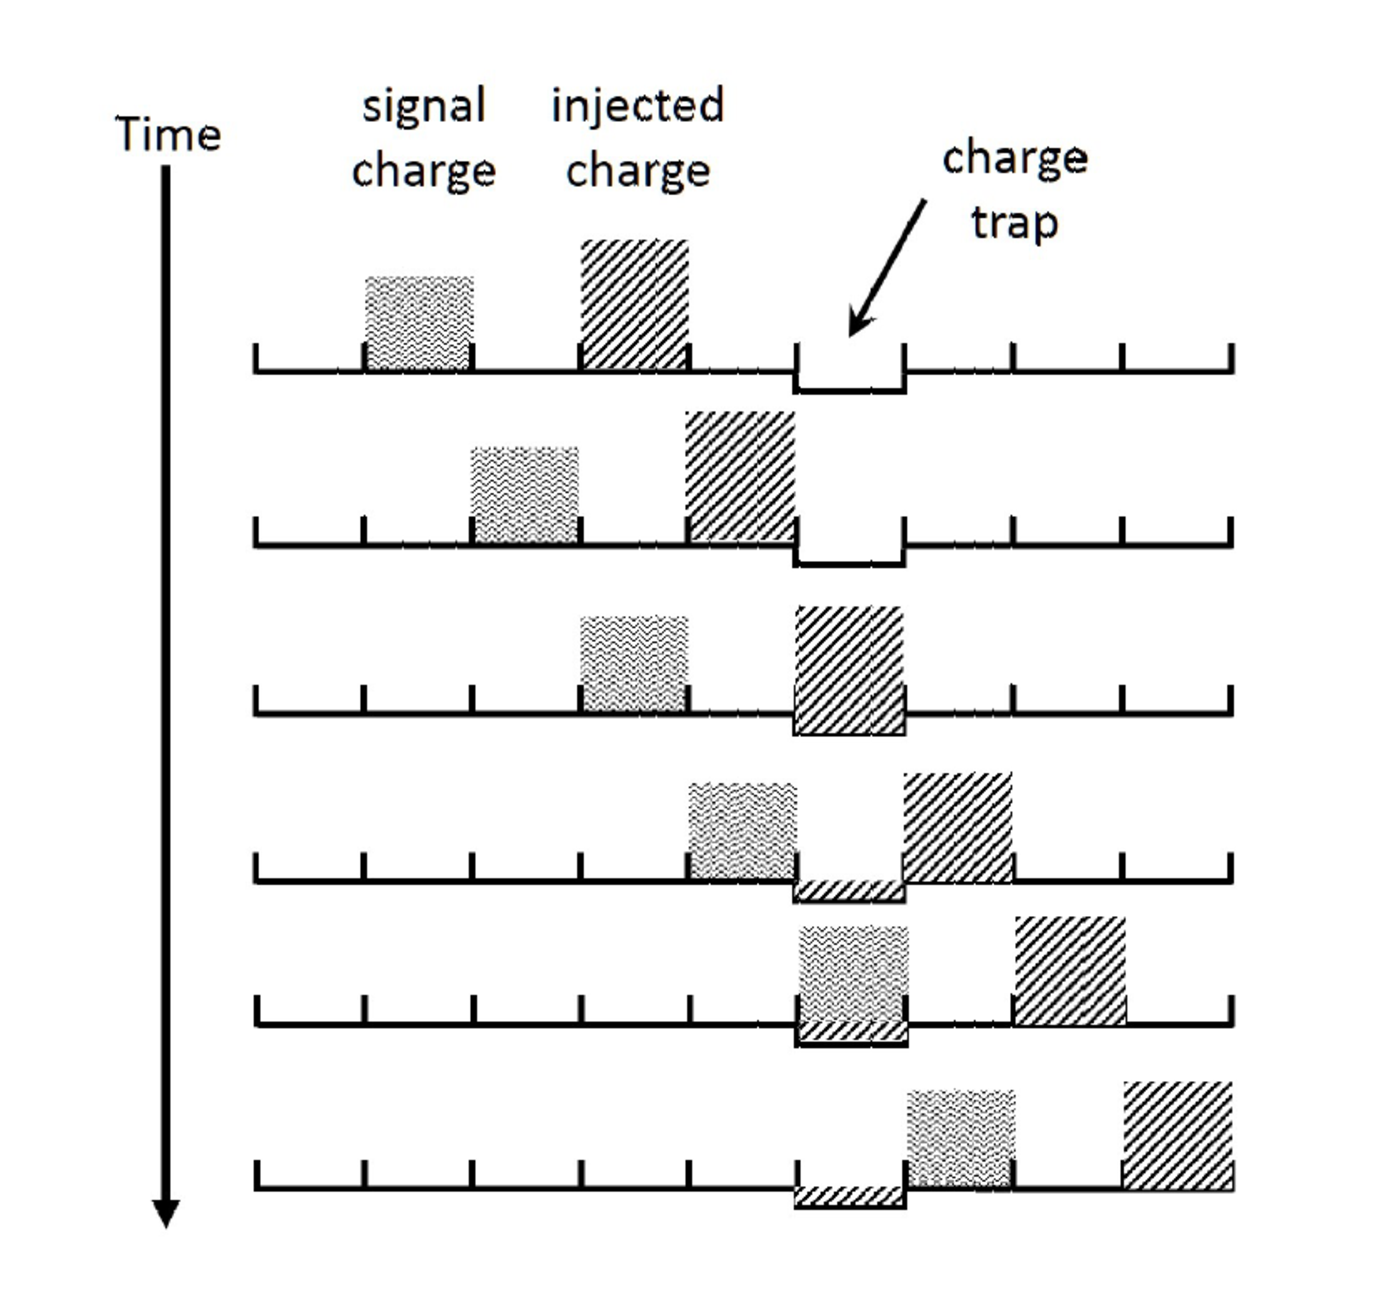
\includegraphics[width=70mm]{Chapter3/Figures/CI-kinou.eps} 
		\caption{CI を注入してトラップによる電荷損失を改善する概念図\cite{ah-jaxa}}
		\label{fig:sxi_ci_transfer}
	\end{center}
\end{figure}

\newpage
\section{静止気象衛星 GOES}

\begin{figure}[H]
	\begin{center}
		\includegraphics[width=100mm,angle=0]{Chapter3/Figures/GOES_satelite.jpg}
	\end{center}
	\caption{GOES衛星(GOES-16) の外観\cite{NOAA}。宇宙天気の観測に太陽紫外線撮像装置(SUVI)、宇宙環境現地観測装置(SEISS)、磁力計(MAG)、極端紫外線とX線放射センサー(EXIS)が使われている。太陽のX線フラックスを観測しているのが、EXISを構成しているX線センサー(XRS)である。}
	\label{fig:GOES_satelite}
\end{figure}

静止気象衛星 GOES (Geostationary Operational Environmental Satelite) は、アメリカ合衆国の静止気象衛星シリーズである。1975年に最初のGOES衛星(GOES-1)が打ち上げられ、2024年に19機目(GOES-19)が打ち上げられた。現在も運用されている GOES-16 の外観を図~\ref{fig:GOES_satelite}に示す。GOESは、地球の西半球の画像撮影や大気測定、リアルタイムの雷活動のマッピング、太陽活動と宇宙天気のモニタリングを行っている。GOESは、静止軌道(赤道上空 3万5800 km) を周回し、地球の自転と同じ速度で運行している。
GOESはアメリカ航空宇宙局(NASA)が開発と打ち上げを担当し、アメリカ海洋大気庁(NOAA)によって運用されている。

	GOES-16には以下6つの装置が搭載されている。
\begin{enumerate}
	\item Advanced Baseline Imager (ABI)
	
	\hspace{1em}地球の天気、海洋、環境を画像化する装置。ABI は、2つの可視光チャネル、4つの近赤外線チャネル、10の赤外線チャネルによって異なるスペクトルバンドで地球を観察している。
		
	\item Geostationary Lightning Mapper (GLM)
	
	\hspace{1em}雷を観測する装置。単一チャネルの近赤外線光過渡検出器で雷活動を連続的に測定している。
		
	\item Extreme Ultraviolet and X-ray Irradiance Sensors (EXIS)
	
	\hspace{1em}EXIS には、XRS と EUVS が搭載されている。XRS は太陽のX線フラックス、EUVS は太陽の極端紫外線フラックスを測定する装置。
	
	\item Magnetometer (MAG)
	
	\hspace{1em}地球周辺の磁場を測定する装置。
		
	\item Solar Ultraviolet Imager (SUVI)
	
	\hspace{1em}太陽の紫外線画像を撮影する装置。太陽のコロナや太陽フレア、コロナ質量放出などの現象を監視している。
	
	\item Space Environment In-Situ Suite (SEISS)
	
	\hspace{1em}磁気圏内のプロトン、電子、重イオンのフラックスを監視する装置。
		
\end{enumerate}
	


\subsection{X線センサー(XRS)}


\begin{figure}[H]
	\begin{center}
		\includegraphics[width=100mm,angle=0]{Chapter3/Figures/GOES_XRS.jpg}
	\end{center}
	\caption{GOESのX線センサー(XRS)の断面図。(Thomas et al.2024)\cite{Thomas}}
	\label{fig:GOES_XRS_view}
\end{figure}

図~\ref{fig:GOES_XRS_view}にGOES /XRS の断面図を示す。光学キャビティの外側は、軽い元素でできたアルミニウム(Al)のハウジング(緑)で覆われており、内側の壁は重い元素を含む銅タングステン合金(オレンジ)で作られている。さらに、X線を制御するベリリウム(Be)フィルターや、光を検出するフォトダイオード、測定データを処理する電子回路、視野を調整するバッフルやコリメーター、磁気を利用したアセンブリ(灰色)も含まれている。

表~\ref{tb:GOES_XRS_perform}にGOES /XRS の主な性能を示す。 GOES には2台の XRS が搭載されており、XRS-A では、0.09-0.37 nm、XRS-B では、0.10-0.69nm の波長帯の太陽X線フラックスを観測している。XRS-B で観測された 0.10-0.69 nm(1-8\AA) のエネルギー帯で測定されたX線フラックスをもとに、太陽フレアの等級分けがされる。$ 10^{-8}$ $\mathrm{W/m^2} $ レベルをAクラスとし、一桁ずつX線フラックスが上がるごとに, B, C, M, Xクラスとクラス分けされている。また, X線フラックスの値との対応をとるために、$5.0^{-6}$ $\mathrm{W/m^2} $ のときには、C5.0 クラスと表記される。表~\ref{tb:GOES_XRS_perform}に示す帯域外除去率とは、指定されたスペクトル範囲外の信号をどの程度抑制できるかを示す指標である。放射照度範囲とは、センサーが検出可能な放射照度の範囲である。分解能(3-s,$ \mathrm{W}/\mathrm{m}^2 $)とは、3秒間の平均値として測定される最小の放射照度変化量を示している。数値が小さいほど、微細な変化を検出できる高い分解能を持つことを意味する。精度(3-s,$ \mathrm{W}/\mathrm{m}^2 $)とは、3秒間の平均値として測定される放射照度の測定精度である。放射照度の正確さは、測定された放射照度値が実際の値とどの程度一致しているかを示す指標である。視野角は、センサーの視野角を分単位で示した値である。

\begin{table}[htbp]
	\begin{center}
		\caption{XRSの主な性能(Thomas et al.2024)\cite{Thomas}}
		\label{tb:GOES_XRS_perform}
		\begin{tabular}{ccccc}
			\hline \hline
			パラメータ & XRS-A channel & XRS-B channel\\ \hline
			スペクトル範囲(nm) & 0.09-0.37 & 0.10-0.69  \\
			帯域外除去率(\%) & 2.8\% & 6.3\%  \\
			放射照度範囲($ \mathrm{W}/\mathrm{m}^2 $) & $10^{-9}$ to $10^{-2}$ &  $10^{-9}$ to $10^{-2}$ \\
			分解能(3-s,$ \mathrm{W}/\mathrm{m}^2 $) & $3.0 \times 10^{-10}$ &  $2.5 \times 10^{-10}$ \\			
			精度(3-s,$ \mathrm{W}/\mathrm{m}^2 $) & $3.8 \times 10^{-9}$ & $3.8 \times 10^{-9}$ \\	
			放射照度の正確さ(\%) & 10\% &  10\%\\
			視野角(FOV, arcmin) & $ \pm 70 $ & $ \pm 70 $	
			\\\hline
		\end{tabular}
	\end{center}
\end{table}
\chapter{観測データ}

XRISM /SXI で観測された太陽の地球大気反射X線は、空間的に分解されていない太陽全面の積分された放射である。そのため、活動領域、静穏領域、フレアなど様々な成分から構成されている。しかし、Xクラスの大規模な太陽フレアでは、フレアの放射自体が観測されるX線放射の約90\%から99\%を占めているため、ほぼ純粋なフレアのX線が得られる。また、高いX線フラックスにより、詳細な分光を行うのに十分な光子を得ることができる。そのため、論文では主に大規模なフレアのみに焦点を当てる。

本研究では、XRISM /SXI が2023年10月19日に観測を開始してから、2024年12月31日までの期間における観測データの調査を行った。2023年10月19日から2024年12月31日の期間において、55回のXクラスフレアが発生した。そのうち、XRISM /SXI の昼地球観測時間とフレアピークが一致するものを選別した。使用した昼地球条件は \texttt{"$ELV < 0 \, \& \, NTE\_ELV > 0$"} である。本研究では、7つのXクラスフレアと2つのMクラスフレアを解析で使用した。表\ref{tb:obsdata}に使用したデータを示す。

\begin{table}[htbp]
	\begin{center}
		\caption{解析に使用した観測データ}
		\label{tb:obsdata}
		\begin{tabular}{ccccc}
			\hline \hline
			観測ID & フレアID & フレアクラス & 開始時刻 &  露光時間(秒)\\ \hline
			300056010 & Flare-1 & X1.69 & 2024年5月3日 02:13:59 & 1284 \\
			300056010 & Flare-2 & X1.29 & 2024年5月5日 11:45:30 & 1352 \\
			300056010 & Flare-3 & M8.29 & 2024年5月7日 16:29:28 & 740 \\
			300042020 & Flare-4 & X3.48 & 2024年5月15日 08:30:00 & 596 \\			
			300053010 & Flare-5 & X1.57 & 2024年7月29日 02:23:19 & 1116 \\	
			300053010 & Flare-6 & M5.45 & 2024年7月31日 18:16:14 & 1136 \\
			201104010 & Flare-7 & X9.05 & 2024年10月3日 12:14:00 & 156 \\			
			201120010 & Flare-8 & X1.84 & 2024年10月9日 02:00:58 & 300 \\	
			201035010 & Flare-9 & X3.33 & 2024年10月24日 04:02:06 & 1028 
			 \\\hline
		\end{tabular}
	\end{center}
\end{table}

\newpage
図\ref{fig:Lcurve} の上段に、各フレアの SXI ライトカーブを示す。これらは、4つのSXIセンサーで得られたすべてのイベントを足し合わせたものである。下段に、 GOES のX線ライトカーブを示す。
\begin{figure}[H]
	\centering
	\begin{tabular}{c}
		\begin{minipage}{0.5\hsize}
			\begin{center}
				\includegraphics[width=5.3cm]{Chapter4/Figures/Flare-1_lcurve.png}
				\hspace{20mm} 
			\end{center}
		\end{minipage}
		\begin{minipage}{0.5\hsize}
			\begin{center}
				\includegraphics[width=5.3cm]{Chapter4/Figures/Flare-2_lcurve.png}
				\hspace{20mm} 
			\end{center}
		\end{minipage}
	\end{tabular}
	\centering
	\begin{tabular}{c}
		\begin{minipage}{0.5\hsize}
			\begin{center}
				\includegraphics[width=5.3cm]{Chapter4/Figures/Flare-3_lcurve.png}
				\hspace{20mm} 
			\end{center}
		\end{minipage}
		\begin{minipage}{0.5\hsize}
			\begin{center}
				\includegraphics[width=5.3cm]{Chapter4/Figures/Flare-4_lcurve.png}
				\hspace{20mm} 
			\end{center}
		\end{minipage}
	\end{tabular}
	\centering
	\begin{tabular}{c}
		\begin{minipage}{0.5\hsize}
			\begin{center}
				\includegraphics[width=5.3cm]{Chapter4/Figures/Flare-5_lcurve.png}
				\hspace{20mm} 
			\end{center}
		\end{minipage}
		\begin{minipage}{0.5\hsize}
			\begin{center}
				\includegraphics[width=5.3cm]{Chapter4/Figures/Flare-6_lcurve.png}
				\hspace{20mm} 
			\end{center}
		\end{minipage}
	\end{tabular}		
	\centering
	\begin{tabular}{c}
		\begin{minipage}{0.5\hsize}
			\begin{center}
				\includegraphics[width=5.3cm]{Chapter4/Figures/Flare-7_lcurve.png}
				\hspace{20mm} 
			\end{center}
		\end{minipage}
		\begin{minipage}{0.5\hsize}
			\begin{center}
				\includegraphics[width=5.3cm]{Chapter4/Figures/Flare-8_lcurve.png}
				\hspace{20mm}
			\end{center}
		\end{minipage}
	\end{tabular}
	\raggedright %
	\begin{tabular}{c}
		\begin{minipage}{0.5\hsize}
			\begin{center}
				\includegraphics[width=5.3cm]{Chapter4/Figures/Flare-9_lcurve.jpg}
				\hspace{20mm} 
			\end{center}
		\end{minipage}
	\end{tabular}	
	\caption{上段は、Flare-1 から Flare-9 の XRISM /SXI の光度曲線。下段に GOES X線フラックスを示す。}
	\label{fig:Lcurve}
\end{figure}






\chapter{スペクトル解析}
本章では、まず Flare-1 から Flare-9 を足し合わせて作成したフレアの積分スペクトルから得られた結果を示す。次にフレアのスペクトルから絶対元素組成比の測定方法について説明する。この絶対元素組成比の測定方法を用いて、フレアクラス別に算出した絶対元素組成比を 5.3 に、フレアピーク付近を時間分割して算出した絶対元素組成比を 5.4 に示す。

\section{積分スペクトル}

\begin{figure}[H]
	\begin{center}
		\includegraphics[width=100mm,angle=0]{Chapter5/Figures/merge_flare_spec.jpg}
	\end{center}
	\caption{Flare-1 から Flare-9 を足し合わせ、プレフレアを差し引いたスペクトル(4つのSXIを合計したもの)。灰色でプレフレアのスペクトルを示す。TI,Cr,Ni は K20\cite{Katsuda} と比較して、SXIで新たに得られた輝線である。}
	\label{fig:flare_merge_spec}
\end{figure}
図\ref{fig:flare_merge_spec} に Flare-1からFlare-9までを足し合わせ、プレフレアを差し引いたスペクトルを示す。基礎となる連続的な放射の上に、Si, S, Ar, Ca, Ti, Cr, Fe, Ni の輝線が得られた。 Ti, Cr, Ni の輝線は \mbox{Katsuda et al.~2020\cite{Katsuda}} と比較して新たに得られた輝線である。以降は Katsuda et al.~2020\cite{Katsuda} を K20 と略する。


\section{絶対元素組成比の測定手法}

\subsection{等価幅の測定}
本研究のスペクトル解析手法は、基本的に K20\cite{Katsuda} に倣ったものである。
太陽X線放射のスペクトル形状は、地球の大気散乱によって変化する。昼地球のデータを解析する際には、このスペクトルの変形を考慮する必要がある。そのため、観測データからスペクトルの変形に影響されない等価幅を測定し、絶対元素組成比に変換した。スペクトルフィッティングの際に使用した Respoonse Matrix File (RMF)と Ancillary Response File(ARF) はそれぞれ xtdrmf 及び xaarfgen を使用して生成した。RMF と ARF の詳細については、Ishisaki et al.2007 \cite{Ishisaki} に記載されている。

\subsection{等価幅から絶対元素組成比への変換}

本節では、等価幅から絶対元素組成比に変換する解析手法を説明する。等価幅は、元素組成比だけでなく温度や電離状態にも依存する。そのため、モデルで期待される等価幅を算出し、これを測定値と比較することで元素組成比を算出した。以下の2つのモデルを使用した。1つは温度 $T$ と放射量 (EM) の2つの値を持つ2温度モデルである。もう一つは、温度に対する微分放射量 (DEM) がべき乗則に従う多温度モデルを採用した (EM = 定数 $\times T^\alpha$)。具体的には、原子データベースの \texttt{ATOMDB 3.1.0} を用いて、\texttt{XSPEC} の2つの \texttt{vapec} モデルを2温度モデルに、1つの \texttt{cevmkl} モデルを多温度モデルに使用した。

2温度モデルでは、温度 ($kT$) を $0.5~\mathrm{keV}$ と $1.7~\mathrm{keV}$ とした。これは、ピーク温度がこれらの値を持つ二峰性の微分放射量を示した先行研究 (Caspi et al.~2014\cite{Caspi}; Sylwester et al.~2014\cite{Sylwester}) に基づく。また、多温度モデルに関しては、Si, S, Ar, Ca の He-like, H-like イオンからの輝線が $0.2 \sim 2~\mathrm{keV}$ の温度範囲の熱プラズマによって形成される。さらに、Xクラスのフレアでは、超高温 ($kT \geq 3~\mathrm{keV}$) の成分が存在する (e.g., Caspi \& Lin 2010)。本研究では、Si, S, Ar, Ca に加え Fe の絶対元素組成比を算出するために、$kT_\mathrm{max}$ を $3.5~\mathrm{keV}$ としてモデル等価幅を測定した。

2温度モデル ($0.5~\mathrm{keV} + 1.7~\mathrm{keV}$) および多温度モデルの場合、等価幅 (EW) は元素組成比だけでなく、2成分の正規化比 ($N_2/N_1$) や温度分布のべき乗指数 ($\alpha$) にも依存する。そのため、等価幅を絶対的な元素組成比に変換するには、これらのパラメータを特定する必要がある。これらのパラメータは、同じ元素の異なる電荷状態に由来する輝線の強度比に敏感であるため、強度比によって測定できる。K20\cite{Katsuda}に倣い、本研究でも、データ内で最も統計のよい \mbox{Si Ly$\alpha$ / Si He$\alpha$} の強度比を選択した。図\ref{fig:flare_alpha_N2divN1}は、Si Ly$\alpha$ / Si He$\alpha$ 比が $N_2/N_1$ および $\alpha$ にどのように依存するかを示している。具体的には、まず2温度モデルで、\texttt{XSPEC} の \texttt{fakeit} を使用して、モデル $vapec+vapec$ の温度を $1.7~\mathrm{keV}$ と $0.5~\mathrm{keV}$ に、$N_1$ を10に固定し、$N_2$ を $0.1$ から $40$ まで $0.01$ ずつ変化させたときの2温度モデルスペクトルを作成した。次に、多温度モデルでも同様に、\texttt{fakeit} を使用して、モデル \texttt{cevmkl} の$kT_\mathrm{max}$ を $3.5~\mathrm{keV}$ に固定してシミュレートを行い、$\alpha$ を $-4$ から $3$ まで $0.01$ ずつ変化させたときの多温度モデルスペクトルを作成した。作成した2温度モデルと多温度モデルスペクトルの Si He$\alpha$ と Si Ly$\alpha$ を、ガウシアンとべき乗モデルでフィットを行い、$N_2/N_1$, $\alpha$ の値における Si Ly$\alpha$ / Si He$\alpha$ の強度比をプロットしたものが図\ref{fig:flare_alpha_N2divN1}である。この図~\ref{fig:flare_alpha_N2divN1}を用いて、各スペクトルごとに、測定した Si Ly$\alpha$ / Si He$\alpha$ から $N_2/N_1$, $\alpha$ の値を決定した。

\begin{figure}[H]
	\centering
	\begin{tabular}{c}
		\begin{minipage}{0.5\hsize}
			\begin{center}
				\includegraphics[width=8cm]{Chapter5/Figures/vapec_0a5and1a7keV_sxi_N1divN2_vs_SiLy_div_SiHe.jpg}
				\hspace{10mm}
			\end{center}
		\end{minipage}
		\begin{minipage}{0.5\hsize}
			\begin{center}
				\includegraphics[width=8cm]{Chapter5/Figures/cevmkl_2keV_sxi_alpha_vs_SiLy_div_SiHe.jpg}
				\hspace{10mm}
			\end{center}
		\end{minipage}
	\end{tabular}
	\caption{左図:2温度モデルの Si Ly$\alpha$ / Si He$\alpha$ の強度比。右図:多温度モデルで、$kT_\mathrm{max}$$3.5~\mathrm{keV}$ でシミュレートした Si Ly$\alpha$ / Si He$\alpha$ の強度比。}
\label{fig:flare_alpha_N2divN1}
\end{figure}

Si Ly$\alpha$ / He$\alpha$ は地球大気反射 (スペクトル硬化の影響)により増加する。この効果を考慮するために、\mbox{K20\cite{Katsuda}} ではモンテカルロシミュレーションを行っている。このシミュレーションでは、入力が太陽X線スペクトル ($kT = 1.5~\mathrm{keV}$ の典型的な太陽フレア温度をもつ\texttt{apec}モデル) であり、出力は地球大気反射スペクトルである。K20\cite{Katsuda} によるシミュレーション結果より、固有の Si Ly$\alpha$ / Si He$\alpha$ は観測値の $0.8$ 倍であると示された。本研究では、K20\cite{Katsuda} と同様に、観測値の $0.8$ 倍で補正を行った。
モデル等価幅は、各スペクトル (Flare 1-9) について、最適な $N_2/N_1$ (2温度モデル) または $\alpha$ (多温度モデル) の条件下で、絶対組成比の関数として算出した。原理的には、モデル等価幅は放射モデル (\texttt{vapec} および \texttt{cevmkl}) から直接導出できる。しかし、本研究では、等価幅の測定と同じように、ガウシアンとべき関数モデルでシミュレートされたSXIスペクトルをフィッティングすることでモデル等価幅を測定した。このプロセスは、特に個々の輝線を分解できない中程度のスペクトル分解能を持つX線CCDにとって重要である。図~\ref{fig:EW_abund}は、例として、Flare-1, Flare-4, Flare-7 の多温度モデルに基づく等価幅を、絶対組成比の関数として示したものである。具体的には、1つ目のプロセスとして、Si Ly$\alpha$ / Si He$\alpha$ の値から図~\ref{fig:flare_alpha_N2divN1}を用いて、各フレアの$\alpha$を測定した。次に測定した$\alpha$でモデル \texttt{cevmkl} の温度を固定し、Si He$\alpha$, Si Ly$\alpha$, S He$\alpha$, S Ly$\alpha$, Ar He$\alpha$, Ca He$\alpha$, Fe He$\alpha$ の絶対元素組成比を $0.01$ から  まで $0.01$ ずつ変化させたときの多温度モデルスペクトルを作成した。作成した多温度モデルスペクトルを $gaussian$ と $powerlaw$ でフィッティングし、各輝線の絶対元素組成比に対する等価幅を算出した値をプロットしたグラフが図~\ref{fig:EW_abund}である。

\begin{figure}[H]
	\centering
	\begin{tabular}{c}
		\begin{minipage}{0.5\hsize}
			\begin{center}
				\includegraphics[width=7cm]{Chapter5/Figures/Si_He_abund_EW.jpg}
				\hspace{40mm}
			\end{center}
		\end{minipage}
		\begin{minipage}{0.5\hsize}
			\begin{center}
				\includegraphics[width=7cm]{Chapter5/Figures/Si_Ly_abund_EW.jpg}
				\hspace{40mm}
			\end{center}
		\end{minipage}
	\end{tabular}
	%CCD2
	\centering
	\begin{tabular}{c}
		\begin{minipage}{0.5\hsize}
			\begin{center}
				\includegraphics[width=7cm]{Chapter5/Figures/S_He_abund_EW.jpg}
				\hspace{40mm}
			\end{center}
		\end{minipage}
		\begin{minipage}{0.5\hsize}
			\begin{center}
				\includegraphics[width=7cm]{Chapter5/Figures/S_Ly_abund_EW.jpg}
				\hspace{40mm}
			\end{center}
		\end{minipage}
	\end{tabular}
	%CCD3
	\centering
	\begin{tabular}{c}
		\begin{minipage}{0.5\hsize}
			\begin{center}
				\includegraphics[width=7cm]{Chapter5/Figures/Ar_He_abund_EW.jpg}
				\hspace{40mm}
			\end{center}
		\end{minipage}
		\begin{minipage}{0.5\hsize}
			\begin{center}
				\includegraphics[width=7cm]{Chapter5/Figures/Ca_He_abund_EW.jpg}
				\hspace{40mm}
			\end{center}
		\end{minipage}
	\end{tabular}		
	%CCD4
	\raggedright %
	\begin{tabular}{c}
		\begin{minipage}{0.5\hsize}
			\begin{center}
				\includegraphics[width=7cm]{Chapter5/Figures/Fe_He_abund_EW.jpg}
				\hspace{40mm}
			\end{center}
		\end{minipage}
	\end{tabular}
	\caption{Si He$\alpha$, Si Ly$\alpha$, S He$\alpha$, S Ly$\alpha$, Ar He$\alpha$, Ca He$\alpha$, Fe He$\alpha$ の絶対元素組成比の関数としての等価幅。これらは多温度モデルに基づいており、温度勾配パラメータ($\alpha$)は、それぞれ Flare-1 ,Flare-4 ,Flare-7 の \mbox{Si Ly$\alpha$ / Si He$\alpha$} から求めた $\alpha$ の値に固定している、データポイントの散布は、シミュレートスペクトルのスペクトル適合から生じる統計的変動である。 }
	\label{fig:EW_abund}
\end{figure}

\newpage
\section{フレアクラス別の絶対元素組成比}
\label{sec:flare_to_falre_abund}
本節では、フレアクラス別に算出した絶対元素組成比の結果を示す。

\begin{figure}[H]
	\centering
	\begin{tabular}{c}
		\begin{minipage}{0.5\hsize}
			\begin{center}
				\includegraphics[width=5.1cm]{Chapter5/Figures/Flare-1_spec.jpg}
				\hspace{5mm}
			\end{center}
		\end{minipage}
		\begin{minipage}{0.5\hsize}
			\begin{center}
				\includegraphics[width=5.1cm]{Chapter5/Figures/Flare-2_spec.jpg}
				\hspace{5mm} 
			\end{center}
		\end{minipage}	
	\end{tabular}	
	\centering
	\begin{tabular}{c}			
		\begin{minipage}{0.5\hsize}
			\begin{center}
				\includegraphics[width=5.1cm]{Chapter5/Figures/Flare-3_spec.jpg}
				\hspace{5mm}
			\end{center}
		\end{minipage}
		\begin{minipage}{0.5\hsize}
			\begin{center}
				\includegraphics[width=5.1cm]{Chapter5/Figures/Flare-4_spec.jpg}
				\hspace{5mm}
			\end{center}
		\end{minipage}																		
	\end{tabular}
	\centering
	\begin{tabular}{c}							
		\begin{minipage}{0.5\hsize}
			\begin{center}
				\includegraphics[width=5.1cm]{Chapter5/Figures/Flare-5_spec.jpg}
				\hspace{5mm} 
			\end{center}
		\end{minipage}
		\begin{minipage}{0.5\hsize}
			\begin{center}
				\includegraphics[width=5.1cm]{Chapter5/Figures/Flare-6_spec.jpg}
				\hspace{5mm}
			\end{center}
		\end{minipage}
	\end{tabular}		
	\centering
	\begin{tabular}{c}							
		\begin{minipage}{0.5\hsize}
			\begin{center}
				\includegraphics[width=5.1cm]{Chapter5/Figures/Flare-8_spec.jpg}
				\hspace{5mm} 
			\end{center}
		\end{minipage}
		\begin{minipage}{0.5\hsize}
			\begin{center}
				\includegraphics[width=5.1cm]{Chapter5/Figures/Flare-9_spec.jpg}
				\hspace{5mm}
			\end{center}
		\end{minipage}		
	\end{tabular}
	\caption{Flare-1 から Flare-9 までの SXI スペクトル(Flare-7 はフレアピークと観測期間がずれていたため、ここでは除外している)。上段に、赤色で $gaussian$ と $powerlaw$ で構成された最適フィットモデルとデータを示す。灰色のデータはバックグラウンドとして使用したプレフレアスペクトルである。下段にフィットモデルとの残差を示す。}
	\label{fig:Flare_spec}
\end{figure}
図~\ref{fig:Flare_spec} にフレアピークを観測した8つのフレアスペクトルを示す。なお、GOESX線フラックスが極大となった時間をフレアピークとしている。ここでは、フレアピークと観測期間がずれていた Flare-7 を除外し、2回のMクラス、4回のX1クラス、2回のX3クラスのフレアを使用した。黒と灰色で示したデータは、それぞれフレアスペクトルとバックグラウンドとして使用したプレフレアスペクトルである。赤色で12のガウス分布とべき乗モデルで構成された最適フィットモデルを示す。



\begin{table}[htbp]
	\begin{center}
		\caption{ガウシアンと連続スペクトルモデルから算出した等価幅(単位は eV )}
		\label{tb:flare_EW}
		\begin{tabular}{ccccccccc}
			\hline \hline
			フレアID & フレアクラス & Si He$\alpha$ &  Si Ly$\alpha$ & S He$\alpha$ & S Ly$\alpha$ & Ar He$\alpha$ & Ca He$\alpha$ & Fe He$\alpha$\\ \hline
			Flare-1 & X1.69 & $145^{+6}_{-8}$ & $76^{+6}_{-5}$ & $74^{+8}_{-8}$ & $28^{+7}_{-8}$ & $44^{+15}_{-13}$ & $108^{+13}_{-15}$ & $952^{+40}_{-63}$ \\
			Flare-2 & X1.29 & $108^{+5}_{-6}$ & $53^{+5}_{-4}$ & $92^{+7}_{-7}$ & $37^{+7}_{-5}$ & $80^{+14}_{-10}$ & $89^{+10}_{-12}$ & $840^{+52}_{-30}$ \\
			Flare-3 & M8.29 & $168^{+8}_{-8}$ & $73^{+8}_{-6}$ & $114^{+9}_{-15}$ & $33^{+10}_{-10}$ & $87^{+19}_{-20}$ & $128^{+19}_{-22}$ & $995^{+86}_{-82}$ \\
			Flare-4 & X3.48 & $77^{+10}_{-7}$ & $103^{+12}_{-10}$ & $42^{+10}_{-12}$ & $24^{+8}_{-9}$ & $26^{+11}_{-12}$ & $159^{+20}_{-15}$ & $1484^{+55}_{-55}$ \\			
			Flare-5 & X1.57 & $178^{+7}_{-8}$ & $88^{+5}_{-6}$ & $118^{+7}_{-7}$ & $36^{+6}_{-7}$ & $63^{+12}_{-11}$ & $115^{+12}_{-12}$ & $1181^{+64}_{-59}$  \\	
			Flare-6 & M5.45 & $111^{+9}_{-8}$ & $44^{+6}_{-6}$ & $94^{+10}_{-9}$ & $37^{+8}_{-8}$ & $99^{+23}_{-19}$ & $157^{+13}_{-26}$ & $799^{+94}_{-82}$ \\		
			Flare-7 & X1.84 & $226^{+8}_{-7}$ & $87^{+5}_{-5}$ & $158^{+8}_{-9}$ & $38^{+7}_{-8}$ & $49^{+10}_{-14}$ & $113^{+19}_{-13}$ & $847^{+68}_{-63}$ \\	
			Flare-9 & X3.33 & $180^{+6}_{-6}$ & $75^{+4}_{-5}$ & $147^{+7}_{-7}$ & $66^{+8}_{-8}$ & $69^{+16}_{-10}$ & $166^{+12}_{-14}$ & $827^{+72}_{-66}$
			\\\hline
		\end{tabular}
	\end{center}
\end{table}
表~\ref{tb:flare_EW} に Flare-1 から Flare-9 を $gaussian$ と $powerlaw$ でフィッティングし、測定した等価幅を示す。


\begin{table}[htbp]
	\begin{center}
		\caption{Si Ly$\alpha$ / Si He$\alpha$ の強度比と図~\ref{fig:flare_alpha_N2divN1}のプロットを用いて求めた $N_2/N_1$ (2温度モデル)、$\alpha$ (多温度モデル)}
		\label{tb:flare_SiLydivSiHe}
		\begin{tabular}{cccccc}
			\hline \hline
			フレアID & フレアクラス & Si Ly$\alpha$/Si He$\alpha$ & Si Ly$\alpha$/Si He$\alpha$ (アルベド補正後) & $\alpha$ & $N_2/N_1$ \\ \hline
			Flare-1 & X1.69 & $0.43\pm0.04$ & $0.35\pm0.03$ & $-0.7^{+0.13}_{-0.13}$ & $0.46^{+0.04}_{-0.05}$ \\
			Flare-2 & X1.29 & $0.41\pm0.04$ & $0.32\pm0.03$ & $-0.79^{+0.12}_{-0.13}$ & $0.43^{+0.04}_{-0.05}$\\
			Flare-3 & M8.29 & $0.35\pm0.04$ & $0.28\pm0.03$ & $-0.99^{+0.11}_{-0.16}$ & $0.36^{+0.04}_{-0.04}$\\
			Flare-4 & X3.48 & $1.22\pm0.18$ & $0.97\pm0.14$ & $0.8^{+0.20}_{-0.24}$ & $1.87^{+0.54}_{-0.43}$\\
			Flare-5 & X1.57 & $0.40\pm0.03$ & $0.32\pm0.02$ & $-0.79^{+0.09}_{-0.11}$ & $0.43^{+0.03}_{-0.04}$\\
			Flare-6 & M5.45 & $0.32\pm0.05$ & $0.25\pm0.04$ & $-1.13^{+0.19}_{-0.21}$ & $0.32^{+0.06}_{-0.05}$\\
			Flare-7 & X1.84 & $0.30\pm0.02$ & $0.24\pm0.02$ & $-1.19^{+0.09}_{-0.08}$ & $0.31^{+0.02}_{-0.02}$\\
			Flare-9 & X3.33 & $0.33\pm0.02$ & $0.26\pm0.02$ & $-1.07^{+0.08}_{-0.09}$ & $0.34^{+0.02}_{-0.02}$
			\\\hline
		\end{tabular}
	\end{center}
\end{table}
表~\ref{tb:flare_SiLydivSiHe} に Si Ly$\alpha$ / Si He$\alpha$ の強度比と図~\ref{fig:flare_alpha_N2divN1}のプロットを用いて求めた $N_2/N_1$ (2温度モデル)、$\alpha$ (多温度モデル)を示す。特に Flare-4 の X3.48 のフレアでは、Si Ly$\alpha$ / Si He$\alpha$ の強度比が他のフレアと比較して大きく、高温成分が顕著にスペクトルに寄与していると考えられる。


\newpage

\begin{table}[htbp]
	\begin{center}
		\caption{フレア別に測定した絶対元素組成比}
		\label{tb:flare_abund}
		\begin{tabular}{cccccccccc}
			\hline \hline
			フレアID(放出モデル) & フレアクラス & Si He$\alpha$ & Si Ly$\alpha$ & S He$\alpha$ & Ar He$\alpha$ & Ca He$\alpha$ & Fe He$\alpha$ \\ \hline
			Flare-1(多温度) & X1.69 & $1.02^{+0.04}_{-0.06}$ & $1.08^{+0.1}_{-0.08}$ & $0.68^{+0.07}_{-0.07}$ & $0.82^{+0.35}_{-0.33}$ & $2.64^{+0.37}_{-0.41}$ & $0.91^{+0.03}_{-0.09}$\\
			Flare-1(2温度) & X1.69 & $0.88^{+0.03}_{-0.05}$ & $0.91^{+0.1}_{-0.05}$ & $0.53^{+0.06}_{-0.08}$ & $0.62^{+0.28}_{-0.27}$ & $2.08^{+0.31}_{-0.34}$ & $1.23^{+0.11}_{-0.09}$ \\
			Flare-2(多温度) & X1.29 & $0.73^{+0.04}_{-0.04}$ & $0.79^{+0.07}_{-0.06}$ & $0.81^{+0.07}_{-0.08}$ & $1.72^{+0.28}_{-0.35}$ & $2.14^{+0.23}_{-0.34}$ & $0.79^{+0.05}_{-0.07}$\\
			Flare-2(2温度) & X1.29 & $0.65^{+0.03}_{-0.04}$ & $0.69^{+0.04}_{-0.06}$ & $0.65^{+0.04}_{-0.06}$ & $1.33^{+0.23}_{-0.21}$ & $1.68^{+0.15}_{-0.25}$ & $0.99^{+0.09}_{-0.13}$ \\
			Flare-3(多温度) & M8.29 & $1.04^{+0.05}_{-0.05}$ & $1.1^{+0.13}_{-0.07}$ & $0.95^{+0.07}_{-0.12}$ & $1.75^{+0.57}_{-0.37}$ & $3.08^{+0.50}_{-0.54}$ & $0.96^{+0.19}_{-0.09}$\\
			Flare-3(2温度) & M8.29 & $0.92^{+0.04}_{-0.05}$ & $0.98^{+0.09}_{-0.07}$ & $0.8^{+0.03}_{-0.13}$ & $1.47^{+0.24}_{-0.49}$ & $2.49^{+0.36}_{-0.42}$ & $1.45^{+0.32}_{-0.28}$\\
			Flare-4(多温度) & X3.48 & $1.38^{+0.19}_{-0.09}$ & $1.49^{+0.17}_{-0.14}$ & $0.73^{+0.15}_{-0.20}$ & $0.49^{+0.40}_{-0.40}$ & $4.89^{+0.10}_{-0.44}$ & $2.26^{+0.53}_{-0.23}$\\
			Flare-4(2温度) & X3.48 & $1.01^{+0.14}_{-0.08}$ & $1.02^{+0.13}_{-0.09}$ & $0.45^{+0.07}_{-0.11}$ & $0.26^{+0.07}_{-0.23}$ & $3.18^{+0.38}_{-0.36}$ & $2.75^{+0.96}_{-0.18}$\\
			Flare-5(多温度) & X1.57 & $1.21^{+0.04}_{-0.06}$ & $1.29^{+0.05}_{-0.09}$ & $1.03^{+0.08}_{-0.06}$ & $1.23^{+0.31}_{-0.24}$ & $2.79^{+0.33}_{-0.34}$ & $1.37^{+0.10}_{-0.15}$\\
			Flare-5(2温度) & X1.57 & $1.05^{+0.04}_{-0.05}$ & $1.12^{+0.03}_{-0.08}$ & $0.83^{+0.04}_{-0.07}$ & $0.98^{+0.18}_{-0.27}$ & $2.23^{+0.15}_{-0.23}$ & $1.97^{+0.30}_{-0.08}$\\
			Flare-6(多温度) & M5.45 & $0.65^{+0.05}_{-0.04}$ & $0.71^{+0.08}_{-0.07}$ & $0.75^{+0.08}_{-0.13}$ & $2.05^{+0.63}_{-0.47}$ & $3.74^{+0.40}_{-0.69}$ & $0.74^{+0.15}_{-0.10}$\\
			Flare-6(2温度) & M5.45 & $0.59^{+0.04}_{-0.04}$ & $0.65^{+0.07}_{-0.08}$ & $0.64^{+0.05}_{-0.08}$ & $1.66^{+0.46}_{-0.31}$ & $3.11^{+0.24}_{-0.56}$ & $0.95^{+0.15}_{-0.23}$\\
			Flare-8(多温度) & X1.84 & $1.3^{+0.05}_{-0.04}$ & $1.4^{+0.08}_{-0.09}$ & $1.24^{+0.06}_{-0.08}$ & $0.88^{+0.18}_{-0.30}$ & $2.61^{+0.49}_{-0.31}$ & $0.83^{+0.09}_{-0.10}$\\
			Flare-8(2温度) & X1.84 & $1.17^{+0.05}_{-0.03}$ & $1.27^{+0.06}_{-0.10}$ & $1.06^{+0.05}_{-0.07}$ & $0.69^{+0.22}_{-0.31}$ & $2.19^{+0.44}_{-0.26}$ & $1.07^{+0.34}_{-0.09}$\\
			Flare-9(多温度) & X3.33 & $1.07^{+0.04}_{-0.04}$ & $1.16^{+0.05}_{-0.06}$ & $1.18^{+0.07}_{-0.05}$ & $1.35^{+0.4}_{-0.23}$ & $4.0^{+0.38}_{-0.37}$ & $0.76^{+0.12}_{-0.10}$\\
			Flare-9(2温度) & X3.33 & $0.96^{+0.03}_{-0.04}$ & $1.04^{+0.05}_{-0.07}$ & $1.01^{+0.03}_{-0.07}$ & $1.04^{+0.35}_{-0.19}$ & $3.35^{+0.19}_{-0.27}$ & $1.03^{+0.17}_{-0.20}$
			\\\hline
		\end{tabular}
	\end{center}
\end{table}
表~\ref{tb:flare_abund} に各フレアの絶対元素組成比を示す。表~\ref{tb:flare_abund}で算出した値は、表~\ref{tb:flare_SiLydivSiHe} で求めた $N_2/N_1$ (2温度モデル)、$\alpha$ (多温度モデル) の値を用いて、図~\ref{fig:EW_abund} と同様にフレアの絶対元素組成比に対する等価幅のプロットを作成し、等価幅から絶対元素組成比に変換した値である。元素組成比の誤差は、等価幅の誤差の範囲内で変動させることによって見積もった。元素組成比は、Lodders(2003)\cite{Lodders}による光球組成比を基準としており、それぞれ Si/H = $3.47 \times 10^{-5}$、S/H = $1.55 \times 10^{-5}$、Ar/H = $3.55 \times 10^{-6}$、Ca/H = $2.19 \times 10^{-6}$、Fe/H = $2.91 \times 10^{-5}$、である。

表~\ref{tb:flare_abund}より、Si He$\alpha$ と Si Ly$\alpha$ に基づく Si の元素組成比が概ね一致していることを確認した。これは、等価幅から元素組成比へ変換するプロセスの信頼性を示している。また、多温度モデルと2温度モデルから求めた元素組成比も概ね一致しており、仮定した放射モデルの安定性を裏付けている。

\newpage


\begin{figure}[H]
	\begin{center}
		\includegraphics[width=120mm,angle=0]{Chapter5/Figures/flare_FIP_Abund_err.jpg}
	\end{center}
	\caption{FIP に対する絶対元素組成比。黒十字で示す値は、 K20\cite{Katsuda} で算出された絶対元素組成比である。これらの組成比は、多温度モデルから導出した値である。Si 組成比は Si He$\alpha$ の値に、S の組成比は S He$\alpha$ に基づいている。}
	\label{fig:flare_fip_abund}
\end{figure}
図~\ref{fig:flare_fip_abund}は、多温度モデルから測定した各フレアの絶対元素組成比を、第一電離ポテンシャル (FIP) を横軸にプロットしたグラフである。黒十字は、 K20\cite{Katsuda} で算出された Xクラスフレアの平均絶対元素組成比の値である。

本研究の解析結果では、Ca, Si, S, Ar の絶対元素組成比がK20\cite{Katsuda}で算出された絶対元素組成比よりも高い値となった。絶対元素組成比が高く見積もられた原因として、元素組成比の測定に使用したフレアクラスの違いが大きく影響していると考えられる。K20\cite{Katsuda} で使われた4つのフレアは、X17.0, X5.4, X6.2, X9.0 であり、本研究で使用した X1 クラスや、X3 クラスのフレアと比べて、より高いクラスのフレアが対象となっている。また、K20\cite{Katsuda}と比較して、多温度モデルのべき乗温度指数 $\alpha$ の値にも違いが顕著に現れた。K20\cite{Katsuda}で算出された4つのフレアの $\alpha$ の値は、$0.44$, $0.27$, $0.80$, $1.62$ である。一方、本研究で算出したフレアの $\alpha$ の値は、Flare-4 を除いて、$-1.19 から -0.7$ の値であった。$\alpha$ の差異は、元素組成比の算出に使用したフレアクラスの違いと 多温度モデルの $kT_\mathrm{max}$ の違いが影響していると考えられる。K20\cite{Katsuda}では、多温度モデルの $kT_\mathrm{max}$ を 2keV で絶対元素組成比の算出を行っているが、本研究では、Fe の絶対元素組成比を求めるために $kT_\mathrm{max}$ を 3.5keV で算出した。

本研究で得られた Ca, Si, S, Ar の組成パターンは、K20\cite{Katsuda} 同様に Si と S の間に``折り返し''を持つ i-FIP を示している(Osten et al. 2003\cite{Osten}, Sanz-Forcada et al. 2003\cite{Sanz-Forcada})。実際に、太陽フレアにおけるこのような i-FIP効果は、高FIP元素が豊富なコロナと、低FIP元素が豊富なコロナでは、フレア中にそれぞれ逆の傾向を示す。つまり低FIP元素が相対的に増加するか、高FIP元素が相対的に増加する(Nordon \& Behar 2008\cite{Nordon})。ただし、Nordon \& Behar 2008\cite{Nordon}の提案は主に Chandora や XMM-Newtomn による恒星観測に基づいているが、その中で太陽も低FIP元素が豊富なコロナを持ち、フレア時には高FIP元素が相対的に強くなる例である。

本研究で新たに算出した Fe の絶対元素組成比は、Flare-4(X3.48) 以外のフレアで 0.76-1.37 という値が得られた。これは、FIP が近い Si と同様の結果である。太陽フレア中に Fe の組成比が増加することが、Warren(2014)\cite{Warren}によって、報告されている。Warren(2014)\cite{Warren}は、Solar Dynamics Observatory/EUV
Variability Experiment を用いて、M9.3からX6.9クラスの21個のフレアの絶対組成比を測定し、Fe の増加を確認した。我々は、XRISM /SXI によるフレア観測でも同様に、フレアピークで Fe の絶対元素組成比が増加することを確認した。一方で、((e.g., Narendranath et al. 2014\cite{Narendranath}, Dennis et al. 2015\cite{Dennis},
Sylwester et al. 2015\cite{Sylwester}) などの研究では、多くの太陽フレアでこのような低FIP元素の増加は観測されなかった。この違いの理由は明らかではないが、本研究およびWarren(2014)\cite{Warren}の対象としたフレアは、他の研究と比較して規模の大きいフレアを対象としていることが要因と考えられる。


\newpage
\section{フレアピーク付近における絶対元素組成比の時間変動}
\label{sec:flare_peak_abund}
フレアピーク付近の観測データを20秒から2分程度の間隔で時間分割し、元素組成比を測定した。時間分割に使用した観測は、特に明るいフレアである、X1.69 の Flare -1, X3.48 の Flare-4, X9.05 の Flare-7 を使用した。
		
		
\begin{figure}[H]
	\centering
	\begin{minipage}{0.48\textwidth}  % 左側(図)
		\centering
		\includegraphics[width=7cm]{Chapter5/Figures/flare-1_lcurve.jpg}
		\caption{Flare-1 を時間分割して色分けした光度曲線}
		\label{fig:flare-1_slice_lcurve}
	\end{minipage}
	\hfill
	\begin{minipage}{0.48\textwidth}  % 右側(表)
		\centering
		\caption{Flare-1を時間分割した観測データ} % ← ここを変更
		\label{tab:Flare-1_slice_data}
		\begin{tabular}{ccc}
			\hline \hline
			フレアID(色分け) & 開始時刻 & 露光時間(秒) \\\hline
			Flare-1a(黒) & 5月3日 02:18:00 & 180 \\
			Flare-1b(青) & 5月3日 02:21:00 & 180 \\
			Flare-1c(赤) & 5月3日 02:24:00 & 180 \\
			Flare-1d(紫) & 5月3日 02:27:00 & 180 \\		
		\end{tabular}
	\end{minipage}
\end{figure}


\begin{figure}[H]
	\centering
	\begin{tabular}{c}
		\begin{minipage}{0.5\hsize}
			\begin{center}
				\includegraphics[width=5.8cm]{Chapter5/Figures/Flare-1a_spec.jpg}
				\hspace{5mm}
			\end{center}
		\end{minipage}
		\begin{minipage}{0.5\hsize}
			\begin{center}
				\includegraphics[width=5.8cm]{Chapter5/Figures/Flare-1b_spec.jpg}
				\hspace{5mm} 
			\end{center}
		\end{minipage}
	\end{tabular}	
	\centering
	\begin{tabular}{c}			
		\begin{minipage}{0.5\hsize}
			\begin{center}
				\includegraphics[width=5.8cm]{Chapter5/Figures/Flare-1c_spec.jpg}
				\hspace{5mm}
			\end{center}
		\end{minipage}
		\begin{minipage}{0.5\hsize}
			\begin{center}
				\includegraphics[width=5.8cm]{Chapter5/Figures/Flare-1d_spec.jpg}
				\hspace{5mm}
			\end{center}
		\end{minipage}			
	\end{tabular}
	\caption{Flare-1 を4つに時間分割したスペクトル}
	\label{fig:Flare-1_slice_spec}
\end{figure}
図~\ref{fig:flare-1_slice_lcurve}に Flare-1 を4つに時間分割して色分けした光度曲線を示す。図~\ref{fig:Flare-1_slice_spec}は、時間分割した4つのスペクトルである。フレアピークで、Ca や Si の強度が強くなっている様子がスペクトルから確認できる。

\newpage

\begin{figure}[H]
	\centering
	\begin{minipage}{0.48\textwidth}  % 左側(図)
		\centering
		\includegraphics[width=7cm]{Chapter5/Figures/flare-4_lcurve.jpg}
		\caption{Flare-4 を時間分割して色分けした光度曲線}
		\label{fig:flare-4_slice_lcurve}
	\end{minipage}
	\hfill
	\begin{minipage}{0.48\textwidth}  % 右側(表)
		\centering
		\caption{Flare-4 を時間分割した観測データ}
		\begin{tabular}{ccc}
			\hline \hline
			フレアID(色分け) & 開始時刻 & 露光時間(秒) \\\hline
			Flare-4a(黒) & 5月15日 08:30:00 & 120 \\
			Flare-4b(青) & 5月15日 08:32:00 & 120 \\
			Flare-4c(赤) & 5月15日 08:34:00 & 120 \\
			Flare-4d(紫) & 5月15日 02:36:00 & 120 \\	
		\end{tabular}
		\label{tab:element_abundance}
	\end{minipage}
\end{figure}

\begin{figure}[H]
	\centering
	\begin{tabular}{c}
		\begin{minipage}{0.5\hsize}
			\begin{center}
				\includegraphics[width=5.8cm]{Chapter5/Figures/Flare-4a_spec.jpg}
				\hspace{5mm}
			\end{center}
		\end{minipage}
		\begin{minipage}{0.5\hsize}
			\begin{center}
				\includegraphics[width=5.8cm]{Chapter5/Figures/Flare-4b_spec.jpg}
				\hspace{5mm} 
			\end{center}
		\end{minipage}
	\end{tabular}	
	\centering
	\begin{tabular}{c}			
		\begin{minipage}{0.5\hsize}
			\begin{center}
				\includegraphics[width=5.8cm]{Chapter5/Figures/Flare-4c_spec.jpg}
				\hspace{5mm}
			\end{center}
		\end{minipage}
		\begin{minipage}{0.5\hsize}
			\begin{center}
				\includegraphics[width=5.8cm]{Chapter5/Figures/Flare-4d_spec.jpg}
				\hspace{5mm}
			\end{center}
		\end{minipage}								
	\end{tabular}
	\caption{Flare-4 を4つに時間分割したスペクトル}
	\label{fig:Flare-4_slice_spec}
\end{figure}
図~\ref{fig:flare-4_slice_lcurve}に Flare-4 を4つに時間分割して色分けした光度曲線を示す。図~\ref{fig:Flare-4_slice_spec}は、時間分割した4つのスペクトルである。Flare-4 は、他のフレアと比較して、特に Si Ly$\alpha$ / Si He$\alpha$ の値が高く、高温成分が顕著にスペクトルに影響していると考えられる。図~\ref{fig:Flare-4_slice_spec}のスペクトルからも、フレアピークに近づくにつれ、Si Ly$\alpha$ の強度が大きくなっていく様子が確認できる。

\newpage


\begin{figure}[H]
	\centering
	\begin{minipage}{0.48\textwidth}  % 左側(図)
		\centering
		\includegraphics[width=7cm]{Chapter5/Figures/flare-8_lcurve.jpg}
		\caption{Flare-8 を時間分割して色分けした光度曲線}
		\label{fig:flare-8_slice_lcurve}
	\end{minipage}
	\hfill
	\begin{minipage}{0.48\textwidth}  % 右側(表)
		\centering
		\caption{Flare-8 を時間分割した観測データ}
		\begin{tabular}{ccc}
			\hline \hline
			フレアID(色分け) & 開始時刻 & 露光時間(秒) \\\hline
			Flare-8a(黒) & 10月3日 12:15:00 & 30 \\
			Flare-8b(青) & 10月3日 12:15:30 & 30 \\
			Flare-8c(赤) & 10月3日 12:16:00 & 20 \\
			Flare-8d(紫) & 10月3日 12:16:20 & 20 
		\end{tabular}
		\label{tab:element_abundance}
	\end{minipage}
\end{figure}

\begin{figure}[H]
	\centering
	\begin{tabular}{c}
		\begin{minipage}{0.5\hsize}
			\begin{center}
				\includegraphics[width=5.8cm]{Chapter5/Figures/Flare-8a_spec.jpg}
				\hspace{5mm}
			\end{center}
		\end{minipage}
		\begin{minipage}{0.5\hsize}
			\begin{center}
				\includegraphics[width=5.8cm]{Chapter5/Figures/Flare-8b_spec.jpg}
				\hspace{5mm} 
			\end{center}
		\end{minipage}
	\end{tabular}	
	\centering
	\begin{tabular}{c}			
		\begin{minipage}{0.5\hsize}
			\begin{center}
				\includegraphics[width=5.8cm]{Chapter5/Figures/Flare-8c_spec.jpg}
				\hspace{5mm}
			\end{center}
		\end{minipage}
		\begin{minipage}{0.5\hsize}
			\begin{center}
				\includegraphics[width=5.8cm]{Chapter5/Figures/Flare-8d_spec.jpg}
				\hspace{5mm}
			\end{center}
		\end{minipage}
	\end{tabular}
	\caption{Flare-8 を時間分割したスペクトル}
	\label{fig:Flare-8_slice_spec}
\end{figure}	
図~\ref{fig:flare-8_slice_lcurve}に Flare-8 を4つに時間分割して色分けした光度曲線を示す。図~\ref{fig:Flare-8_slice_spec}は、時間分割した4つのスペクトルである。Flare-8 は、2024年に XRISM /SXI で観測した最大のフレアである。特に、フレアの立ち上がりに伴って、Ca の強度が高くなっている様子がスペクトルから確認できる。


\newpage

\begin{table}[htbp]
	\begin{center}
		\caption{ガウシアンと連続スペクトルモデルから算出した等価幅(単位は eV )}
		\label{tb:flare_slice_EW}
		\begin{tabular}{ccccccccc}
			\hline \hline
			フレアID  & Si He$\alpha$ &  Si Ly$\alpha$ & S He$\alpha$ & S Ly$\alpha$ & Ar He$\alpha$ & Ca He$\alpha$ & Fe He$\alpha$ \\ \hline
			Flare-1a & $145^{+22}_{-21}$ & $68^{+19}_{-14}$ & $79^{+21}_{-22}$ & $54^{+25}_{-20}$ & $111^{+58}_{-36}$ & $59^{+30}_{-25}$ & $1210^{+164}_{-85}$  \\
			Flare-1b & $135^{+8}_{-14}$ & $84^{+12}_{-10}$ & $67^{+12}_{-11}$ & $39^{+11}_{-11}$ & $24^{+19}_{-11}$ & $117^{+25}_{-21}$ & $924^{+62}_{-71}$ \\
			Flare-1c & $152^{+14}_{-11}$ & $80^{+13}_{-13}$ & $96^{+18}_{-14}$ & $15^{+16}_{-15}$ & $25^{+21}_{-25}$ & $152^{+36}_{-28}$ & $814^{+101}_{-99}$\\
			Flare-1d & $148^{+20}_{-23}$ & $60^{+21}_{-14}$ & $102^{+29}_{-25}$ & $22^{+30}_{-22}$ & $94^{+64}_{-42}$ & $99^{+59}_{-48}$ & $855^{+275}_{-211}$\\		
			Flare-4a & $141^{+37}_{-33}$ & $49^{+29}_{-26}$ & $52^{+41}_{-36}$ & $97^{+31}_{-56}$ & $0^{+43}_{-0}$ & $122^{+41}_{-44}$ & $1197^{+148}_{-153}$\\	
			Flare-4b & $31^{+18}_{-12}$ & $63^{+20}_{-15}$ & $14^{+15}_{-14}$ & $1^{+18}_{-1}$ & $3^{+22}_{-3}$ & $135^{+27}_{-27}$ & $1664^{+67}_{-150}$\\		
			Flare-4c & $89^{+19}_{-16}$ & $157^{+26}_{-26}$ & $72^{+29}_{-17}$ & $36^{+25}_{-20}$ & $67^{+37}_{-34}$ & $235^{+23}_{-33}$ & $1615^{+146}_{-95}$\\	
			Flare-4d & $86^{+19}_{-22}$ & $108^{+19}_{-24}$ & $67^{+23}_{-23}$ & $40^{+24}_{-18}$ & $24^{+29}_{-24}$ & $202^{+33}_{-32}$ & $1342^{+124}_{-142}$\\	
			Flare-8a & $154^{+33}_{-21}$ & $37^{+21}_{-15}$ & $109^{+30}_{-25}$ & $0^{+24}_{-0}$ & $63^{+47}_{-50}$ & $13^{+33}_{-13}$ & $596^{+66}_{-106}$ \\
			Flare-8b & $138^{+20}_{-24}$ & $50^{+17}_{-15}$ & $45^{+16}_{-19}$ & $49^{+18}_{-19}$ & $108^{+40}_{-51}$ & $50^{+29}_{-28}$ & $1113^{+174}_{-119}$ \\
			Flare-8c & $125^{+19}_{-20}$ & $91^{+19}_{-18}$ & $72^{+23}_{-23}$ & $22^{+15}_{-21}$ & $14^{+31}_{-14}$ & $119^{+35}_{-16}$ & $1281^{+101}_{-160}$\\
			Flare-8d & $109^{+17}_{-16}$ & $80^{+12}_{-14}$ & $76^{+22}_{-17}$ & $17^{+18}_{-15}$ & $45^{+22}_{-29}$ & $126^{+26}_{-21}$ & $1046^{+94}_{-96}$ 
			\\\hline
		\end{tabular}
	\end{center}
\end{table}
表~\ref{tb:flare_slice_EW}に時間分割したフレアの Si He$\alpha$, Si Ly$\alpha$, S He$\alpha$, S Ly$\alpha$, Ar He$\alpha$, Ca He$\alpha$, Fe He$\alpha$の等価幅を示す。



\begin{table}[htbp]
	\begin{center}
		\caption{Si Ly$\alpha$ / Si He$\alpha$ の強度比と図~\ref{fig:flare_alpha_N2divN1}のプロットを用いて求めた $N_2/N_1$ (2温度モデル)、$\alpha$ (多温度モデル)}
		\label{tb:flare_slice_SiLydivSiHe}
		\begin{tabular}{cccccc}
			\hline \hline
			フレアID & Si Ly$\alpha$/Si He$\alpha$ & Si Ly$\alpha$/Si He$\alpha$ (アルベド補正後) & $\alpha$ & $N_2/N_1$ \\ \hline
			Flare-1a & $0.4\pm0.11$ & $0.32\pm0.09$ & $-0.8^{+0.33}_{-0.42}$ & $0.43^{+0.13}_{-0.13}$ \\
			Flare-1b & $0.52\pm0.06$ & $0.42\pm0.05$ & $-0.44^{+0.17}_{-0.19}$ & $0.57^{+0.08}_{-0.08}$ \\
			Flare-1c & $0.43\pm0.07$ & $0.34\pm0.06$ & $-0.74^{+0.23}_{-0.24}$ & $0.45^{+0.08}_{-0.08}$ \\
			Flare-1d & $0.33\pm0.10$ & $0.26\pm0.08$ & $-1.08^{+0.36}_{-0.48}$ & $0.34^{+0.11}_{-0.11}$ \\
			Flare-4a & $0.32\pm0.20$ & $0.25\pm0.16$ & $-1.13^{+0.67}_{-1.15}$ & $0.33^{+0.23}_{-0.20}$ \\
			Flare-4b & $1.84\pm1.12$ & $1.48\pm0.90$ & $1.4^{+0.69}_{-1.37}$ & $3.99^{+0.00}_{-3.12}$ \\
			Flare-4c & $1.62\pm0.38$ & $1.3\pm0.30$ & $1.2^{+0.30}_{-0.41}$ & $3.33^{+0.66}_{-1.38}$ \\
			Flare-4d & $1.13\pm0.30$ & $0.9\pm0.24$ & $0.68^{+0.35}_{-0.44}$ & $1.64^{+0.89}_{-0.61}$ \\						
			Flare-8a & $0.21\pm0.11$ & $0.17\pm0.09$ & $-1.66^{+0.54}_{-0.78}$ & $0.21^{+0.12}_{-0.10}$ \\
			Flare-8b & $0.31\pm0.10$ & $0.25\pm0.08$ & $-1.15^{+0.38}_{-0.48}$ & $0.32^{+0.12}_{-0.10}$ \\
			Flare-8c & $0.63\pm0.13$ & $0.5\pm0.10$ & $-0.17^{+0.27}_{-0.32}$ & $0.72^{+0.20}_{-0.18}$ \\
			Flare-8d & $0.64\pm0.13$ & $0.51\pm0.10$ & $-0.14^{+0.28}_{-0.32}$ & $0.73^{+0.21}_{-0.17}$ 
			\\\hline
		\end{tabular}
	\end{center}
\end{table}
表~\ref{tb:flare_slice_SiLydivSiHe}に Si He$\alpha$ / Si He$\alpha$ の強度比と図~\ref{fig:flare_alpha_N2divN1}のプロットを用いて求めた $N_2/N_1$ (2温度モデル)、$\alpha$ (多温度モデル)を示す。表~\ref{tb:flare_slice_SiLydivSiHe} から、時間分割したときの温度成分の変化を知ることができる。特に 大きなフレアが発生した際の Flare-8 に注目すると、Flare-8a から Flare-8d へのフレアの立ち上がりに伴って、温度成分 $\alpha$ の値が大きくなっていき、高温成分がよりフレアピーク付近で影響していることがわかる。

\newpage


\begin{table}[htbp]
	\begin{center}
		\caption{フレア別に測定した絶対元素組成比}
		\label{tb:flare_slice_abund}
		\begin{tabular}{ccccccccc}
			\hline \hline
			フレアID & Si He$\alpha$ & Si Ly$\alpha$ & S He$\alpha$ & Ar He$\alpha$ & Ca He$\alpha$ & Fe He$\alpha$ \\ \hline
			Flare-1a & $0.97^{+0.15}_{-0.14}$ & $1.0^{+0.26}_{-0.19}$ & $0.71^{+0.18}_{-0.19}$ & $2.6^{+1.49}_{-1.00}$ & $1.33^{+0.75}_{-0.53}$ & $1.4^{+0.49}_{-0.16}$\\
			Flare-1b & $1.08^{+0.07}_{-0.10}$ & $1.17^{+0.13}_{-0.14}$ & $0.67^{+0.13}_{-0.09}$ & $0.44^{+0.51}_{-0.41}$ & $2.96^{+0.73}_{-0.62}$ & $0.82^{+0.10}_{-0.08}$\\
			Flare-1c & $1.05^{+0.10}_{-0.09}$ & $1.15^{+0.17}_{-0.19}$ & $0.86^{+0.16}_{-0.12}$ & $0.33^{+0.54}_{-0.31}$ & $3.78^{+0.91}_{-0.74}$ & $0.72^{+0.17}_{-0.11}$\\
			Flare-1d & $0.88^{+0.12}_{-0.14}$ & $0.95^{+0.31}_{-0.20}$ & $0.82^{+0.23}_{-0.19}$ & $1.95^{+1.52}_{-1.00}$ & $2.3^{+1.51}_{-1.17}$ & $0.8^{+0.50}_{-0.26}$\\
			Flare-4a & $0.82^{+0.22}_{-0.19}$ & $0.8^{+0.43}_{-0.38}$ & $0.44^{+0.29}_{-0.28}$ & $0.01^{+0.74}_{-0.00}$ & $2.87^{+1.00}_{-1.08}$ & $1.4^{+0.46}_{-0.23}$\\
			Flare-4b & $0.96^{+0.45}_{-0.26}$ & $1.01^{+0.29}_{-0.20}$ & $0.36^{+0.26}_{-0.32}$ & $0.02^{+0.54}_{-0.00}$ & $4.43^{+0.56}_{-1.10}$ & $3.49^{+0.56}_{-0.93}$\\
			Flare-4c & $2.1^{+0.41}_{-0.37}$ & $2.32^{+0.37}_{-0.36}$ & $1.42^{+0.51}_{-0.34}$ & $2.2^{+1.80}_{-1.40}$ & $4.96^{+0.00}_{-0.00}$ & $3.07^{+1.38}_{-0.60}$\\
			Flare-4d & $1.43^{+0.29}_{-0.36}$ & $1.54^{+0.23}_{-0.33}$ & $1.04^{+0.36}_{-0.31}$ & $0.53^{+0.88}_{-0.52}$ & $4.94^{+0.00}_{-0.00}$ & $1.84^{+0.36}_{-0.30}$\\
			Flare-8a & $0.76^{+0.17}_{-0.10}$ & $0.76^{+0.40}_{-0.27}$ & $0.77^{+0.2}_{-0.05}$ & $1.14^{+0.99}_{-1.06}$ & $0.25^{+0.69}_{-0.24}$ & $0.51^{+0.08}_{-0.11}$\\	
			Flare-8b & $0.8^{+0.12}_{-0.14}$ & $0.81^{+0.25}_{-0.21}$ & $0.38^{+0.13}_{-0.13}$ & $2.24^{+1.04}_{-1.13}$ & $1.09^{+0.69}_{-0.63}$ & $1.26^{+0.44}_{-0.22}$\\	
			Flare-8c & $1.19^{+0.17}_{-0.19}$ & $1.25^{+0.23}_{-0.25}$ & $0.81^{+0.23}_{-0.24}$ & $0.14^{+0.85}_{-0.12}$ & $3.16^{+0.95}_{-0.48}$ & $1.54^{+0.30}_{-0.32}$\\	
			Flare-8d & $1.06^{+0.16}_{-0.15}$ & $1.11^{+0.17}_{-0.19}$ & $0.86^{+0.23}_{-0.18}$ & $0.95^{+0.65}_{-0.77}$ & $3.32^{+0.73}_{-0.57}$ & $1.07^{+0.19}_{-0.17}$									
			\\\hline
		\end{tabular}
	\end{center}
\end{table}
表~\ref{tb:flare_slice_abund} に各フレアの絶対元素組成比を示す。表~\ref{tb:flare_slice_abund}で算出した値は、表~\ref{fig:flare_alpha_N2divN1}で求めた $N_2/N_1$ (2温度モデル)、$\alpha$ (多温度モデル) の値を用いて、図~\ref{fig:EW_abund} と同様にフレアの絶対元素組成比に対する等価幅のプロットを作成し、等価幅から絶対元素組成比に変換した値である。


\begin{figure}[H]
	\centering
	\begin{tabular}{c}
		\begin{minipage}{0.5\hsize}
			\begin{center}
				\includegraphics[width=5.8cm]{Chapter5/Figures/flare_slice_Si.jpg}
				\hspace{5mm}
			\end{center}
		\end{minipage}
		\begin{minipage}{0.5\hsize}
			\begin{center}
				\includegraphics[width=5.8cm]{Chapter5/Figures/flare_slice_S.jpg}
				\hspace{5mm} 
			\end{center}
		\end{minipage}
	\end{tabular}	
	\centering
	\begin{tabular}{c}			
		\begin{minipage}{0.33\hsize}
			\begin{center}
				\includegraphics[width=5.8cm]{Chapter5/Figures/flare_slice_Ar.jpg}
				\hspace{5mm}
			\end{center}
		\end{minipage}
		\begin{minipage}{0.33\hsize}
			\begin{center}
				\includegraphics[width=5.8cm]{Chapter5/Figures/flare_slice_Ca.jpg}
				\hspace{5mm}
			\end{center}
		\end{minipage}
		\begin{minipage}{0.33\hsize}
		\begin{center}
				\includegraphics[width=5.8cm]{Chapter5/Figures/flare_slice_Fe.jpg}
				\hspace{5mm}
			\end{center}
		\end{minipage}		
	\end{tabular}
	\caption{フレアピークの時間を横軸 0 としたときの、Flare-1,Flare-4,Flare-9 を時間分割して求めた絶対元素組成比の時間変化。}
	\label{fig:flare_slice_abund}
\end{figure}
図~\ref{fig:flare_slice_abund}に、Flare-1,Flare-4,Flare-9 を時間分割して求めた Si, S, Ar, Ca, Fe の絶対元素組成比の時間変化を示す。フレアピークの時間を 0 として横軸を設定している。とりわけ Ca は顕著に絶対元素組成比が変化しており、フレアの立ち上がりからフレアピークにかけて、絶対元素組成比が増大している。Si, S, Fe でも フレア立ち上がりから、絶対元素組成比が増大しているが、フレアピーク直前で絶対元素組成比が最大となり、その後は減少していく傾向が見られた。

\chapter{まとめ}
本研究では、X線天文衛星 XRISM に搭載した X線撮像検出器 SXI を用いて、\mbox{2023年10月19日}から\mbox{2024年12月31日}の期間における、太陽フレアの地球大気反射X線の観測を行った。以下に結果をまとめる。

\begin{itemize}
	\item 9つのフレア観測データを足し合わせ、積分スペクトルを作成した。積分したフレアスペクトルから、Si, S, Ar, Ca, Ti, Cr, Fe, Ni の輝線が得られ、Katsuda et al.2020\cite{Katsuda} と比較して、新たに Ti, Cr, Ni の輝線を確認した。
	
	\item フレア毎に絶対元素組成比を測定した。
	\begin{itemize}
		\item 絶対元素組成比を算出したすべてのフレアが i-FIP を示す結果となった。これは、Katsuda et al.2020\cite{Katsuda}と同様の結果である。
		\item Katsuda et al.2020\cite{Katsuda}と比較して、Si, S, Ar, Ca の絶対元素組成比が高い値となった。この原因として、元素組成比の測定に使用したフレアクラスの違いが大きく影響していると考えられる。Katsuda et al.2020{Katsuda} で使われた4つのフレアは、X17.0, X5.4, X6.2, X9.0 であり、本研究で使用した X1 クラスや、X3 クラスのフレアと比べて、高いクラスのフレアが使用されている。
		\item 本研究では新たに、Fe の絶対元素組成比を算出した。結果として、Fe の絶対元素組成比は、ほとんどのフレアで 0.76-1.37 であった。これは FIP の近い Si と同様の結果であり、恒星コロナで観測される FIP 効果と i-FIP 効果の両方を説明する Laming model (Laming et al, 2021\cite{Laming_2021})と整合している。
	\end{itemize}
	\item フレアピーク付近における絶対元素組成比の時間変動を検証した。
	\begin{itemize}
		\item Si , S, Ca の絶対元素組成比は、フレアの立ち上がりから、フレアピークにかけて増大し、フレアピーク以降は減少している傾向が見られた。特に Ca はフレアピーク付近で顕著に変動することが明らかとなった。
	\end{itemize}
\end{itemize}




%%%%%%%%%%%%%%%%%%%%%%%%%%%%%%%%%%%%%%%%%%%%%%%%%%%%%%%%%%%%
% References
%%%%%%%%%%%%%%%%%%%%%%%%%%%%%%%%%%%%%%%%%%%%%%%%%%%%%%%%%%%%
\hypersetup{
	colorlinks=true,
	linkcolor=blue,
	urlcolor=red
}


\begin{thebibliography}{9}
	%Chapter1
	\bibitem{Katsuda} Katsuda et al.2020,
	\href{https://ui.adsabs.harvard.edu/abs/2020ApJ...891..126K/abstract}{ApJ,891,13}
	
	\bibitem{Shimizu}清水敏文, 1998,
	\href{https://www.asj.or.jp/geppou/archive_open/1998/pdf/19980901c.pdf}{天文月報, 91,399}

	\bibitem{Meyer}Meyer, J. P. 1985,
	\href{https://ui.adsabs.harvard.edu/abs/1985ApJS...57..173M/abstract}{ApJS, 57, 173}
	
	\bibitem{Schmelz}Schmelz, J. T., Reames, D. V., von Steiger, R., \& Basu, S. 2012,
	\href{https://ui.adsabs.harvard.edu/abs/2012ApJ...755...33S/abstract}{ ApJ, 755, 33}
	
	\bibitem{Reames}Reames, D. V. 2018, SSRv,
	\href{https://ui.adsabs.harvard.edu/abs/2018SSRv..214...61R/abstract}{ 214, 61}

	\bibitem{Feldman}Feldman, U. 1992,
	\href{https://ui.adsabs.harvard.edu/abs/1992PhyS...46..202F/abstract}{ PhyS, 46, 202}
	
	\bibitem{Dennis}Dennis, B. R., Phillips, K. J. H., Schwartz, R. A., et al. 2015,
	\href{https://ui.adsabs.harvard.edu/abs/2015ApJ...803...67D/abstract}{ ApJ, 803, 67}
	
	
	%2章
	\bibitem{shin_tenmongaku}谷口義明-監修, 新$\cdot$天文学辞典, 2013, 8章
	
	\bibitem{Mitani}三谷夏子, 東京大学大学院修士論文
	\href{https://www-space.eps.s.u-tokyo.ac.jp/group/yokoyama-lab/thesis/2005master_mitani.pdf?utm_source=chatgpt.com}{, 2005}
	
	\bibitem{Lang_1995}``Sun, Earth and Sky'': K. R. Lang, Springer, 1995.
	


	\bibitem{solar_image}JAXA, webページ, 2020, 
	\href{https://www.isas.jaxa.jp/topics/002460.html}{, ``遠くの恒星のように太陽を研究''}
	
	\bibitem{hinode_photosphere}NAOJ, webページ, 2018
	\href{https://hinode.nao.ac.jp/news/column/post-54/}{, ``ひのでが見た太陽表面の模様''}
	
	\bibitem{hinode_sunspot}NAOJ, webページ, 2006
	\href{https://hinode.nao.ac.jp/news/results/post-10/}{, ``ひので搭載可視光$\cdot$磁場望遠鏡の初期成果''}
	
	\bibitem{hinode_sunspot_model}NAOJ, webページ, 2017
	\href{https://hinode.nao.ac.jp/news/topics/post-46/}{, ``ひのでがとらえた大規模フレアとその磁場構造の画像の公開''}
	
	\bibitem{Zurich}国立科学博物館, webページ
	\href{https://www.kahaku.go.jp/research/db/science_engineering/sunspot/zurich.html}{, ``チューリッヒ分類''}
	
	\bibitem{SDO_prominence}JAXA, webページ
	\href{https://www.isas.jaxa.jp/topics/000226.html}{, 日米太陽観測衛星``ひので''``IRIS''の共演}
	
	\bibitem{Kane}Kane et al.1974 
	\href{https://adsabs.harvard.edu/full/1974IAUS...57..105K}{, in IAU Symp. 57: Coronal Disturbances, 105–141}
	
	\bibitem{SOT}JAXA, webページ
	\href{https://www.isas.jaxa.jp/j/special/2008/hinode/13.shtml}{, ``古くて新しい謎、白色光フレア''}
	
	\bibitem{youko_flare_loop}ISAS/JAXA,
	\href{https://www.isas.jaxa.jp/ISASnews/No.262/chap4-03.html}{, ``フレアの磁気リコネクション''}
	
	\bibitem{Shibata}Shibata, K., Masuda, S., Shimojo, M., Hara, H., Yokoyama, T., Tsuneta,S., Kosugi, T., \& Ogawara, Y. 1995
	\href{https://iopscience.iop.org/article/10.1086/309688}{, ApJ, 451, L83}	
	
	\bibitem{SOHO_CME}SOHO webページ
	\href{https://soho.nascom.nasa.gov/bestofsoho/images/las02.html}{, Feb. 27, 2000}
	
	\bibitem{ESA_EUI_FSI}ESA webページ
	\href{https://www.cosmos.esa.int/web/solar-orbiter}{, ``Solar Orbiter''}
	
	\bibitem{solar_system}JAXA webページ
	\href{https://www.isas.jaxa.jp/j/forefront/2010/tsuneta/index.shtml}{, ``46億年の太陽史''}
	
	\bibitem{sunspot_cycle}NASA webページ
	\href{https://solarscience.msfc.nasa.gov/SunspotCycle.shtml}{, ``The Sunspot Cycle''}
	
	\bibitem{Lin}Lin et al., 2002
	\href{https://articles.adsabs.harvard.edu/cgi-bin/nph-iarticle_query?bibcode=2004ESASP.552...45S&db_key=AST&page_ind=5&data_type=GIF&type=SCREEN_VIEW&classic=YES}{Solar Physics, 210, 2}
	
	
	\bibitem{ISAS_NAOJ}国立天文台 webページ
	\href{https://www.nao.ac.jp/news/science/2020/20201009-sso.html}{2020/10/09}
	
	\bibitem{Jaxa_hinode} Jaxa webページ 
	\href{https://www.isas.jaxa.jp/j/special/2008/hinode/13.shtml}{``太陽観測衛星ひので''}
	
	
	%3章
	\bibitem{xrism_sat_overlook}Tashiro, M. et al., 2020,
	\href{https://ui.adsabs.harvard.edu/abs/2020SPIE11444E..22T/abstract}{ Proc. SPIE 11444}
	
	\bibitem{tashiro_2024}Tashiro, M. et al., 2024,
	\href{https://www.spiedigitallibrary.org/conference-proceedings-of-spie/13093/130931G/Development-and-operation-status-of-X-Ray-Imaging-and-Spectroscopy/10.1117/12.3019325.short}{ Proc. SPIE, 13093}
	
	\bibitem{ishisaki_2022}Ishisaki, Y. et al., 2022
	\href{https://www.spiedigitallibrary.org/conference-proceedings-of-spie/12181/121811S/Status-of-resolve-instrument-onboard-X-Ray-Imaging-and-Spectroscopy/10.1117/12.2630654.short?webSyncID=b3444d41-9106-5853-653e-6ce8282b5d45&sessionGUID=a6ee4868-e377-e3c5-734c-ded24b957902}{, Proc. SPIE, 12181}
	
	\bibitem{mori_2022}Mori, K. et al., 2022,
	\href{https://www.spiedigitallibrary.org/conference-proceedings-of-spie/12181/121811T/Xtend-the-soft-x-ray-imaging-telescope-for-the-X/10.1117/12.2626894.short}{ Proc. SPIE, 121811}
	
	
	\bibitem{xrism_pog}ISAS/JAXA, X-ray Astrophisics Laboratory, GSFC, ESA, 2024,
	\href{https://heasarc.gsfc.nasa.gov/docs/xrism/proposals/POG/xrism_pog.pdf}{ The XRISM Proposers' Observatory Guide}
	
	\bibitem{sxi_outlook} 
	\href{https://www.xrism.jaxa.jp/}{X線分光撮像衛星 XRISM, web ページ}
	 
	\bibitem{ah-jaxa} 科学衛星 ASTRO-H 実験計画書, 宇宙科学研究所, 2015

	\bibitem{sxi_name_ref} Hayashida, K., Tomida, H., Mori K., et al.
	\href{https://www.spiedigitallibrary.org/conference-proceedings-of-spie/10699/1069923/Soft-x-ray-imaging-telescope-Xtend-onboard-X-ray-Astronomy/10.1117/12.2311446.short}{ 2018, Proc. of SPIE, 10699, 1069923.}
	
	\bibitem{Tamura_K_2022} Tamura, K., Hayashi, T., Boissay-Malaquin, R., et al. 2022,
	\href{https://www.spiedigitallibrary.org/conference-proceedings-of-spie/12181/121811V/Ground-calibration-of-the-x-ray-mirror-assembly-for-the/10.1117/12.2629534.short}{ Proc. of SPIE, 12181, 121811V.}
	
	
	\bibitem{Kilbourne_2018a}Kilbourne, C. A. et al. 2018a, 	
	\href{https://www.spiedigitallibrary.org/journals/journal-of-astronomical-telescopes-instruments-and-systems/volume-4/issue-01/011214/Design-implementation-and-performance-of-the-Astro-H-SXS-calorimeter/10.1117/1.JATIS.4.1.011214.full}{ Journal of Astronomical Telescopes, Instruments, and Systems, Vol. 4, Issue 1, 011214}
	
	\bibitem{sxi_name_ref} Hayashida, K., Tomida, H., Mori K., et al. 2018,
	\href{https://www.spiedigitallibrary.org/conference-proceedings-of-spie/10699/1069923/Soft-x-ray-imaging-telescope-Xtend-onboard-X-ray-Astronomy/10.1117/12.2311446.short}{ Proc. of SPIE, 10699, 1069923.}

	
	\bibitem{NOAA} NOAA(アメリカ海洋大気庁) ホームページ 
	\href{https://www.nesdis.noaa.gov/news/goes-16-our-newest-and-best-defense-against-the-threats-of-space-weather}{, GOES-16}
	
	\bibitem{Thomas} Thomas N.Woods et al.2024

 
	\bibitem{Caspi} Caspi, A., McTiernan, J. M.,  Warren, H. P. 2014, ApJL, 788, L31
	
	\bibitem{Sylwester} Sylwester, B., Sylwester, J., Phillips, K. J. H., et al. 2014, ApJ, 787, 122
	
	\bibitem{Ishisaki} Ishisaki et al .2007
	
	\bibitem{Drake}Drake, J. J., Laming, J. M., \& Widing, K. G. 1997,
	\href{https://ui.adsabs.harvard.edu/abs/1997ApJ...478..403D/abstract}{ ApJ, 478, 403}
	
	\bibitem{Laming_Drake}Laming, J. M., \& Drake, J. J. 1999,
	\href{https://ui.adsabs.harvard.edu/abs/1999ApJ...516..324L/abstract}{ ApJ, 516, 324}
	
	\bibitem{Brinkman}Brinkman, A. C., Behar, E., Güdel, M., et al. 2001,
	\href{https://ui.adsabs.harvard.edu/abs/2001A%26A...365L.324B/abstract}{ A\&A, 365, L324}
	
	\bibitem{Güdel}Güdel, M., Audard, M., Briggs, K., et al. 2001,
	\href{https://ui.adsabs.harvard.edu/abs/2001A%26A...365L.336G/abstract}{ A\&A, 365, L336}
	
	\bibitem{Audard}Audard, M., Güdel, M., Sres, A., Raassen, A. J. J., \& Mewe, R. 2003, 
	\href{https://www.aanda.org/articles/aa/abs/2003/06/aa3099/aa3099.html}{ A\&A, 398, 1137}
	
	\bibitem{Huenemoerder_2003}Huenemoerder, D. P., Canizares, C. R., Drake, J. J., \& Sanz-Forcada, J. 2003,
	\href{https://ui.adsabs.harvard.edu/abs/2003ApJ...595.1131H/abstract}{ApJ, 595, 1131}
	
	\bibitem{Sanz-Foreada}Sanz-Forcada, J., Maggio, A., \& Micela, G. 2003, 
	\href{https://ui.adsabs.harvard.edu/abs/2003A%26A...408.1087S/abstract}{A\&A, 408, 1087}
	
	\bibitem{Argiroffi}Argiroffi, C., Drake, J. J., Maggio, A., et al. 2004, 
	\href{https://ui.adsabs.harvard.edu/abs/2004ApJ...609..925A/abstract}{ApJ, 609, 925}
	
	\bibitem{Wood_2010}Wood, B. E., \& Linsky, J. L. 2010,
	\href{https://ui.adsabs.harvard.edu/abs/2010ApJ...717.1279W/abstract}{ ApJ, 717, 1279}
	
	\bibitem{Wood_2018}Wood, B. E., Laming, J. M., Warren, H. P., \& Poppenhaeger, K. 2018,
	\href{https://iopscience.iop.org/article/10.3847/1538-4357/aaccf6}{ ApJ, 862, 66}
	
	\bibitem{Huenemoerder_2013}Huenemoerder, D. P., Phillips, K. J. H., Sylwester, J., \& Sylwester, B. 2013,
	\href{https://ui.adsabs.harvard.edu/abs/2013ApJ...768..135H/abstract}{ ApJ, 768, 135}
	
	\bibitem{Laming_2004}Laming, J. M. 2004, ApJ,
	\href{https://ui.adsabs.harvard.edu/abs/2004ApJ...614.1063L/abstract}{ 614, 1063}
	
	\bibitem{Laming_2009}Laming, J. M. 2009,
	\href{https://ui.adsabs.harvard.edu/abs/2009ApJ...695..954L/abstract}{ ApJ, 695, 954}
	
	\bibitem{Laming_2012}Laming, J. M. 2012,
	\href{https://ui.adsabs.harvard.edu/abs/2012ApJ...744..115L/abstract}{ ApJ, 744, 115}
	
	\bibitem{Laming_2015}Laming, J. M. 2015,
	\href{https://ui.adsabs.harvard.edu/abs/2015LRSP...12....2L/abstract}{ LRSP, 12, 2}
	
	\bibitem{Laming_2021}Laming, J. M. 2021,
	\href{https://ui.adsabs.harvard.edu/abs/2021ApJ...909...17L/abstract}{ ApJ, 909 ,17}
	
	\bibitem{Fledman_Widing}Feldman, U., \& Widing, K. G. 1993,
	\href{https://ui.adsabs.harvard.edu/abs/1993ApJ...414..381F/abstract}{ ApJ, 414, 381}
	
	
	\bibitem{Lodders}Lodders, K. 2003,
	\href{https://ui.adsabs.harvard.edu/abs/2003ApJ...591.1220L/abstract}{ ApJ, 591, 1220}
	
	\bibitem{Doscheck}Doschek, G. A., Warren, H. P., \& Feldman, U. 2015,
	\href{https://ui.adsabs.harvard.edu/abs/2015ApJ...808L...7D/abstract}{ ApJL, 808, L7}
	
	\bibitem{Osten}Osten, R. A., Ayres, T. R., Brown, A., et al. 2003,
	\href{https://ui.adsabs.harvard.edu/abs/2003ApJ...582.1073O/abstract}{ ApJ, 582, 1073}
	
	\bibitem{Sanz-Forcada}Sanz-Forcada, J., Maggio, A., \& Micela, G. 2003,
	\href{https://ui.adsabs.harvard.edu/abs/2003A%26A...408.1087S/abstract}{ A\&A, 408, 1087}
	
	\bibitem{Argiroffi}Argiroffi, C., Drake, J. J., Maggio, A., et al. 2004,
	\href{https://ui.adsabs.harvard.edu/abs/2004ApJ...609..925A/abstract}{ ApJ, 609, 925}
	
	\bibitem{Huenemoerder_2013}Huenemoerder, D. P., Phillips, K. J. H., Sylwester, J., \& Sylwester, B. 2013,
	\href{https://ui.adsabs.harvard.edu/abs/2013ApJ...768..135H/abstract}{ ApJ, 768, 135}
	
	\bibitem{Nordon}Nordon, R., \& Behar, E. 2008,
	\href{https://ui.adsabs.harvard.edu/abs/2008A%26A...482..639N/abstract}{ A\&A, 482, 639}
	
	\bibitem{Warren}Warren, H. P. 2014,
	\href{https://ui.adsabs.harvard.edu/abs/2014ApJ...786L...2W/abstract}{ ApJL, 786, L2}
	
	\bibitem{Narendranath}Narendranath, S., Sreekumar, P., Alha, L., et al. 2014,
	\href{https://ui.adsabs.harvard.edu/abs/2014SoPh..289.1585N/abstract}{ SoPh, 289, 1585}
	
	
\end{thebibliography}{}



%%%%%%%%%%%%%%%%%%%%%%%%%%%%%%%%%%%%%%%%%%%%%%%%%%%%%%%%%%%%
% Appendix
%%%%%%%%%%%%%%%%%%%%%%%%%%%%%%%%%%%%%%%%%%%%%%%%%%%%%%%%%%%%
\appendix
\include{Appendix/Appendix}


%%%%%%%%%%%%%%%%%%%%%%%%%%%%%%%%%%%%%%%%%%%%%%%%%%%%%%%%%%%%
% Acknowledges
%%%%%%%%%%%%%%%%%%%%%%%%%%%%%%%%%%%%%%%%%%%%%%%%%%%%%%%%%%%%
%\include{Acknowledgment/Acknowledgment}

\end{document}